% setup
\documentclass{beamer}
\usepackage[utf8]{inputenc}
\usepackage{graphicx}
\usepackage{hyperref}
\usepackage{url}

\usetheme{Boadilla}
\usecolortheme{seahorse}

% footer 
\setbeamertemplate{footline}{
\hbox{\begin{beamercolorbox}[wd=.3\paperwidth,ht=2.25ex,dp=1ex,center]{author in head/foot}
    \usebeamerfont{author in head/foot}\insertshortauthor
  \end{beamercolorbox}%
  
  \begin{beamercolorbox}[wd=.4\paperwidth,ht=2.25ex,dp=1ex,center]{title in head/foot}%
    \usebeamerfont{title in head/foot}
    \insertsection
  \end{beamercolorbox}%
  
  \begin{beamercolorbox}[wd=.3\paperwidth,ht=2.25ex,dp=1ex,right]{author in head/foot}
    \usebeamerfont{author in head/foot}
    \insertframenumber{} / \inserttotalframenumber\hspace*{5ex}
  \end{beamercolorbox}}
}

\begin{document}

% info for title page
\title{Semantic Image Synthesis with\newline  Spatially-Adaptive Normalization}
\subtitle{Taesung Park\textsuperscript{1,2}, Ming-Yu Liu\textsuperscript{2}, Ting-Chun Wang\textsuperscript{2}, Jun-Yan Zhu\textsuperscript{2,3} \newline \textsuperscript{1}UC Berkeley, \textsuperscript{2}NVIDIA ,\textsuperscript{3}MIT CSAIL}
\author{Alexander Koenig, Li Nguyen}
\institute{Workshop in Machine Learning Applications for Computer Graphics \newline Blavatnik School of Computer Science, Tel Aviv University}
\date{April 1, 2020}

% TITLE AND TOC
\frame{\titlepage} 
\frame{\frametitle{Outline}\tableofcontents} 

% INTRODUCTION
\section{Introduction}
\frame{\frametitle{Outline}\tableofcontents[currentsection]}

\begin{frame}
\frametitle{Conditional Image Synthesis}
\begin{itemize}
	\item \textbf{Conditional Image Synthesis}: method to generate photorealistic images based on certain input (e.g. labels, text, ...) 
	\item Semantic Image Synthesis: method to generate photorealistic images based on \textbf{semantic segmentation mask}
\end{itemize}
\begin{figure}
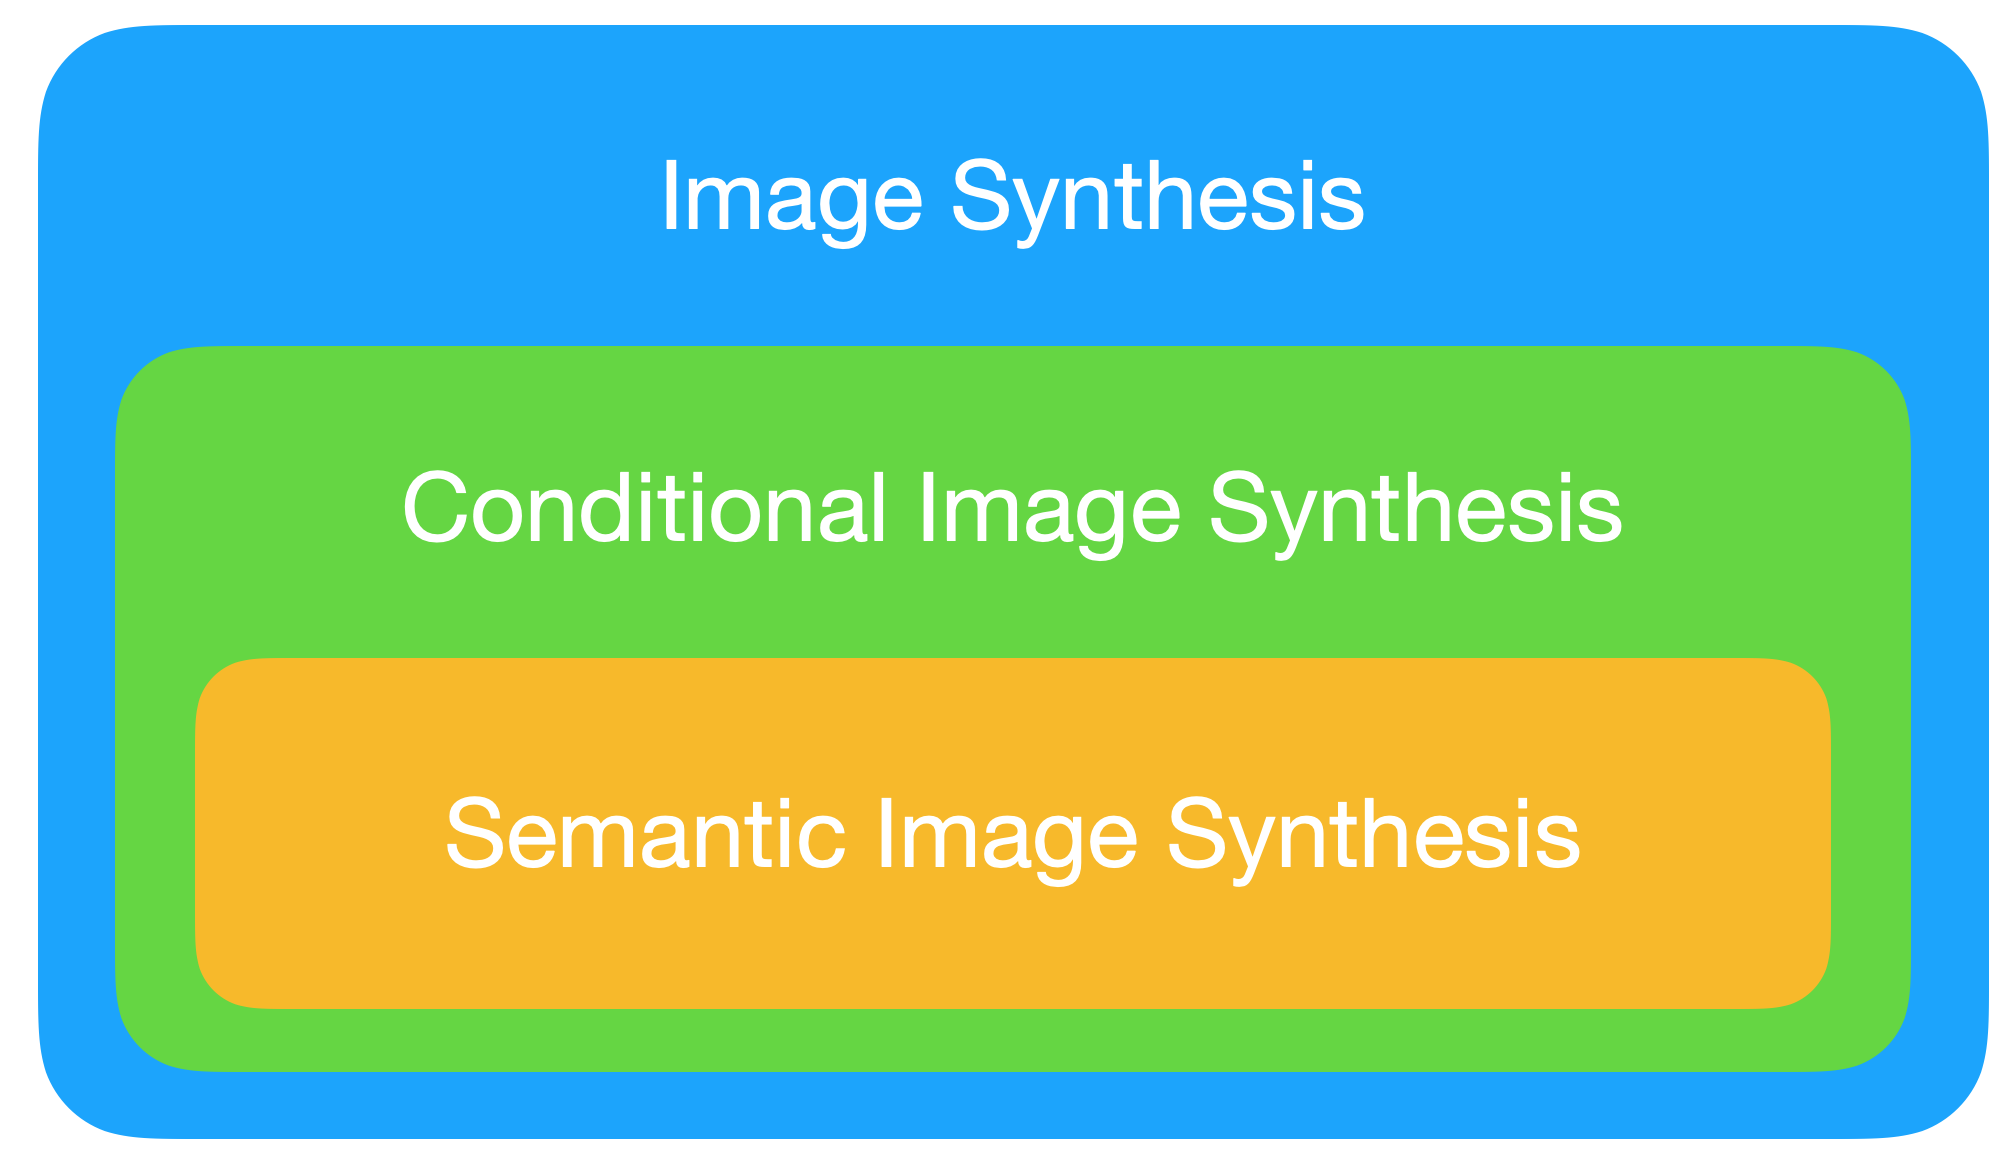
\includegraphics[scale=0.2]{figures/subsets} 
\caption{Euler diagram of image synthesis methods}
\end{figure}
\end{frame}

\begin{frame}
	\frametitle{What is a Semantic Segmentation Mask?}
	
    \begin{figure}
        \begin{minipage}[b]{0.45\linewidth}
            \centering
            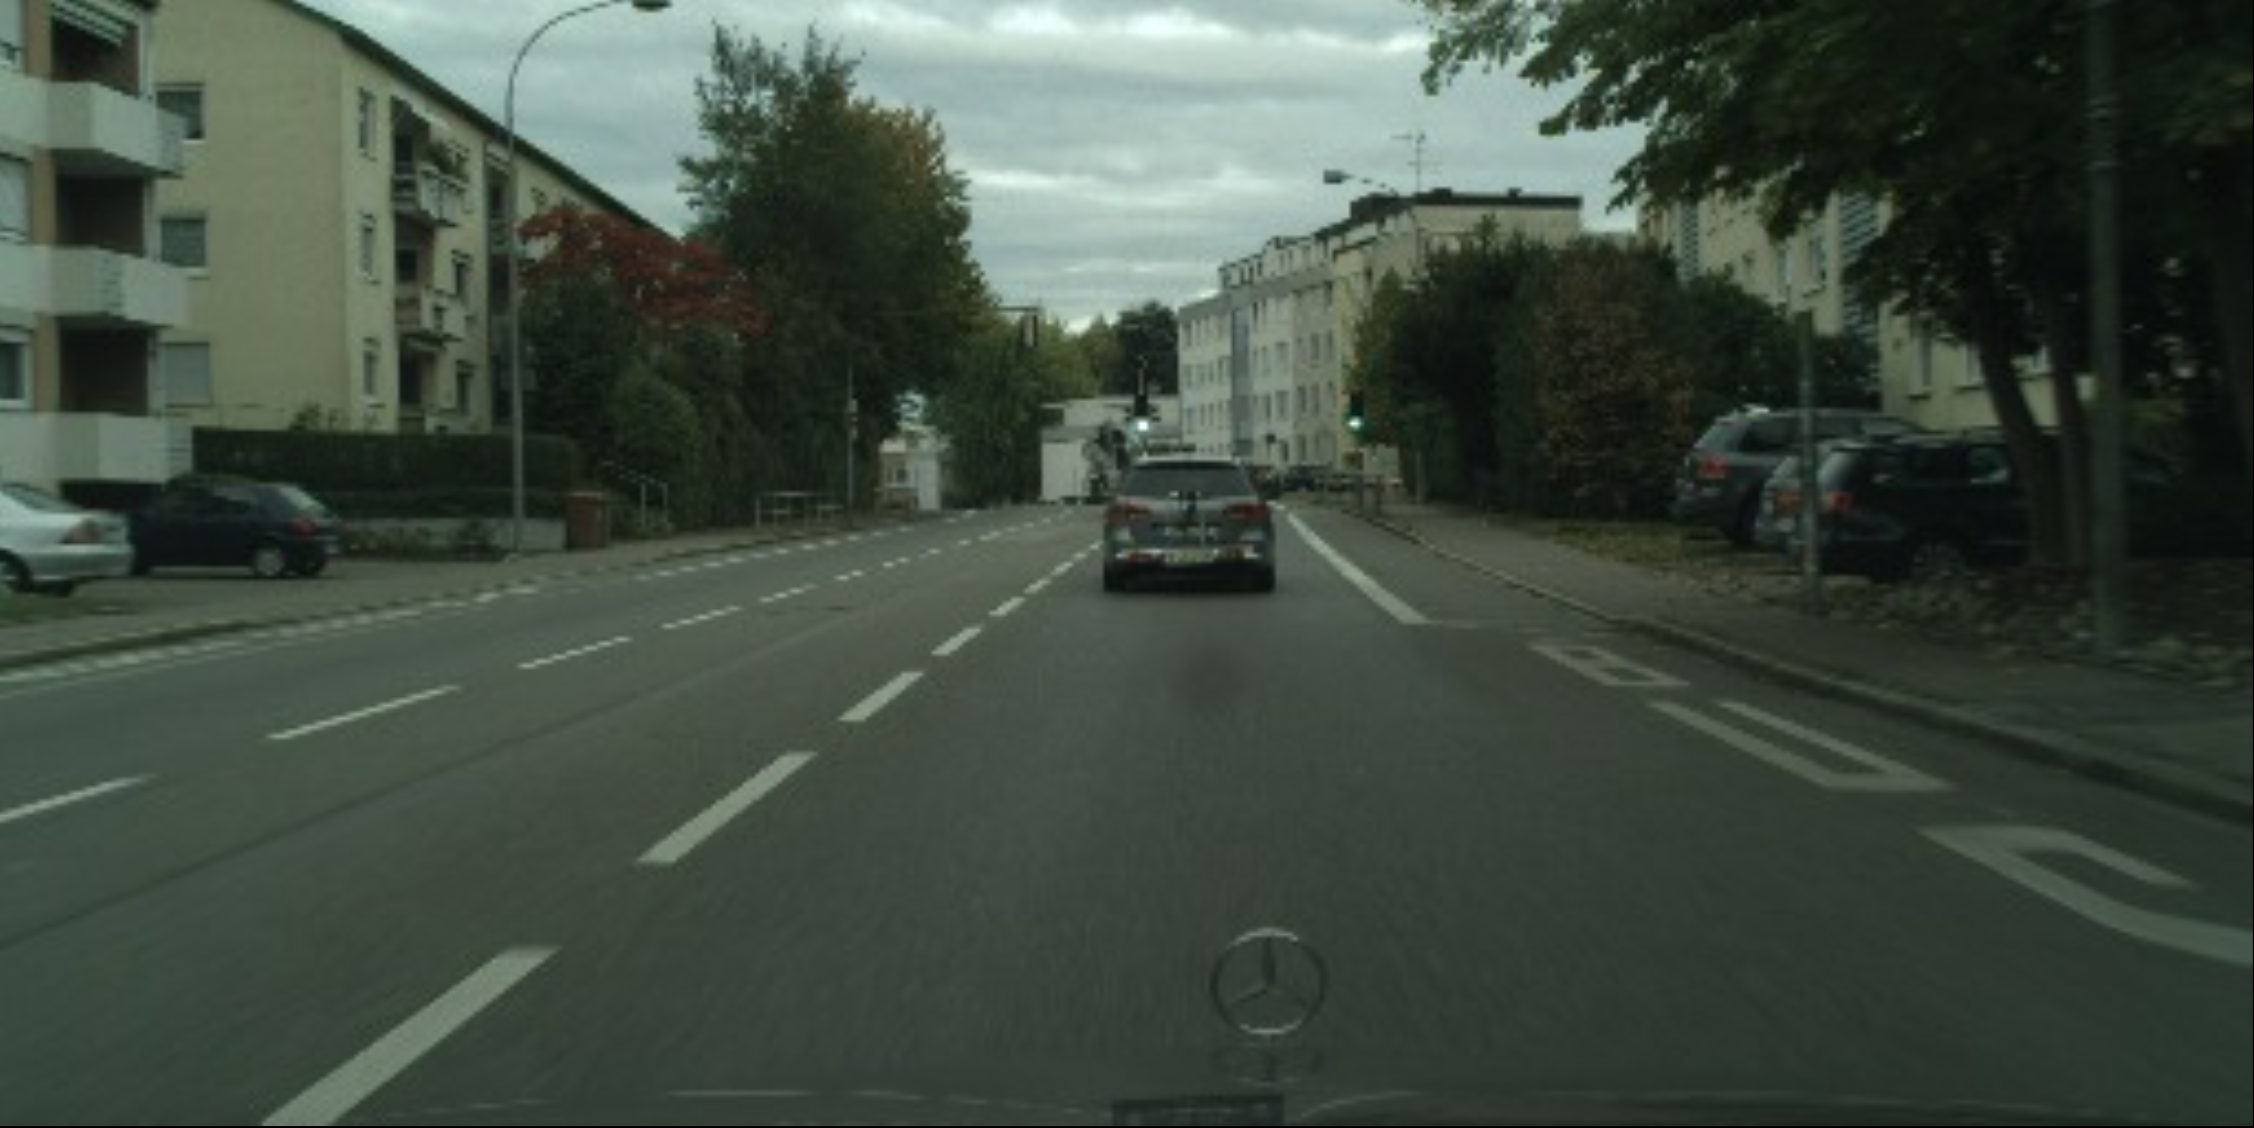
\includegraphics[width=\textwidth]{figures/ground_truth.png}
            \caption{Ground truth \cite{park2019semantic}}
        \end{minipage}
        \hspace{0.5cm}
        \begin{minipage}[b]{0.45\linewidth}
            \centering
            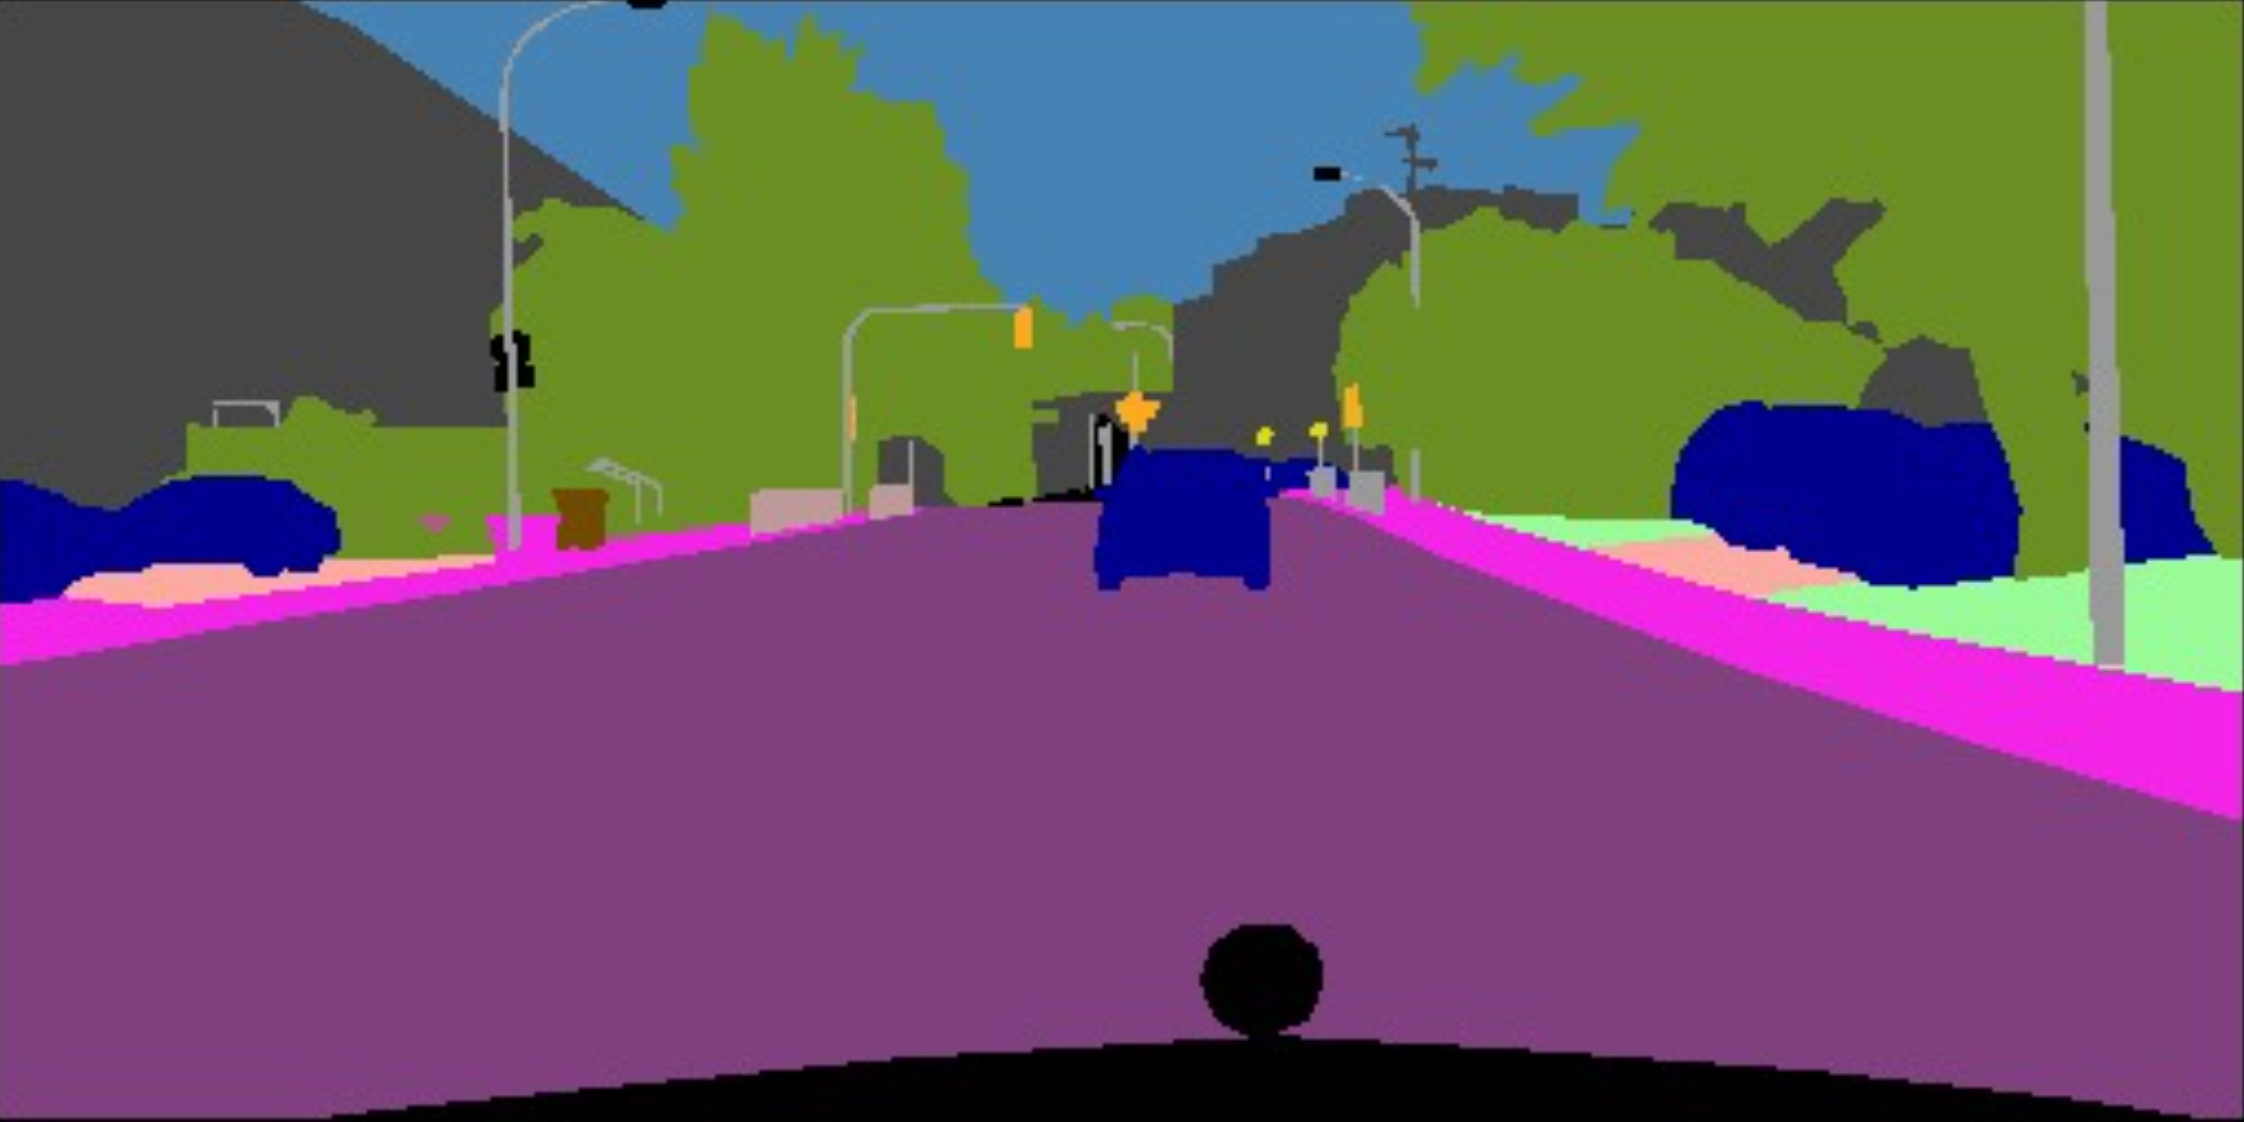
\includegraphics[width=\textwidth]{figures/segmentation.png}
            \caption{Segmentation mask \cite{park2019semantic}}
        \end{minipage}
    \end{figure}
    
    \begin{itemize}
	    \item Semantic segmentation: clustering image pixels together which belong to the same object class \cite{thoma2016survey}
	    \item Goal: turn segmentation mask into a photorealistic image
        \item Application of Semantic Image Synthesis: content generation and image editing
    \end{itemize}
\end{frame}

% RELATED WORK
\section{Related Work}
\frame{\frametitle{Outline}\tableofcontents[currentsection]}

\begin{frame}
\frametitle{Related Work}
\centering
    \begin{figure}
        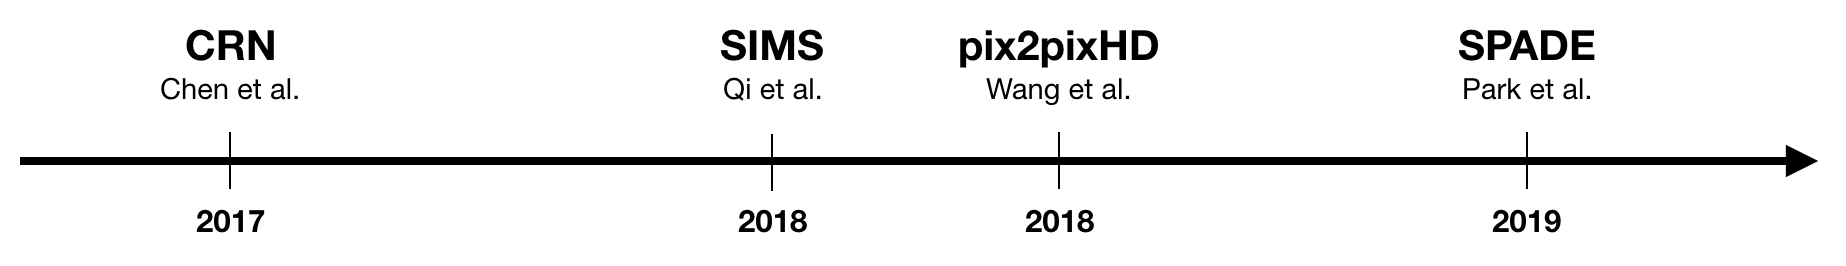
\includegraphics[scale=0.34]{figures/chronology.png} 
    \end{figure}
    \begin{figure}
        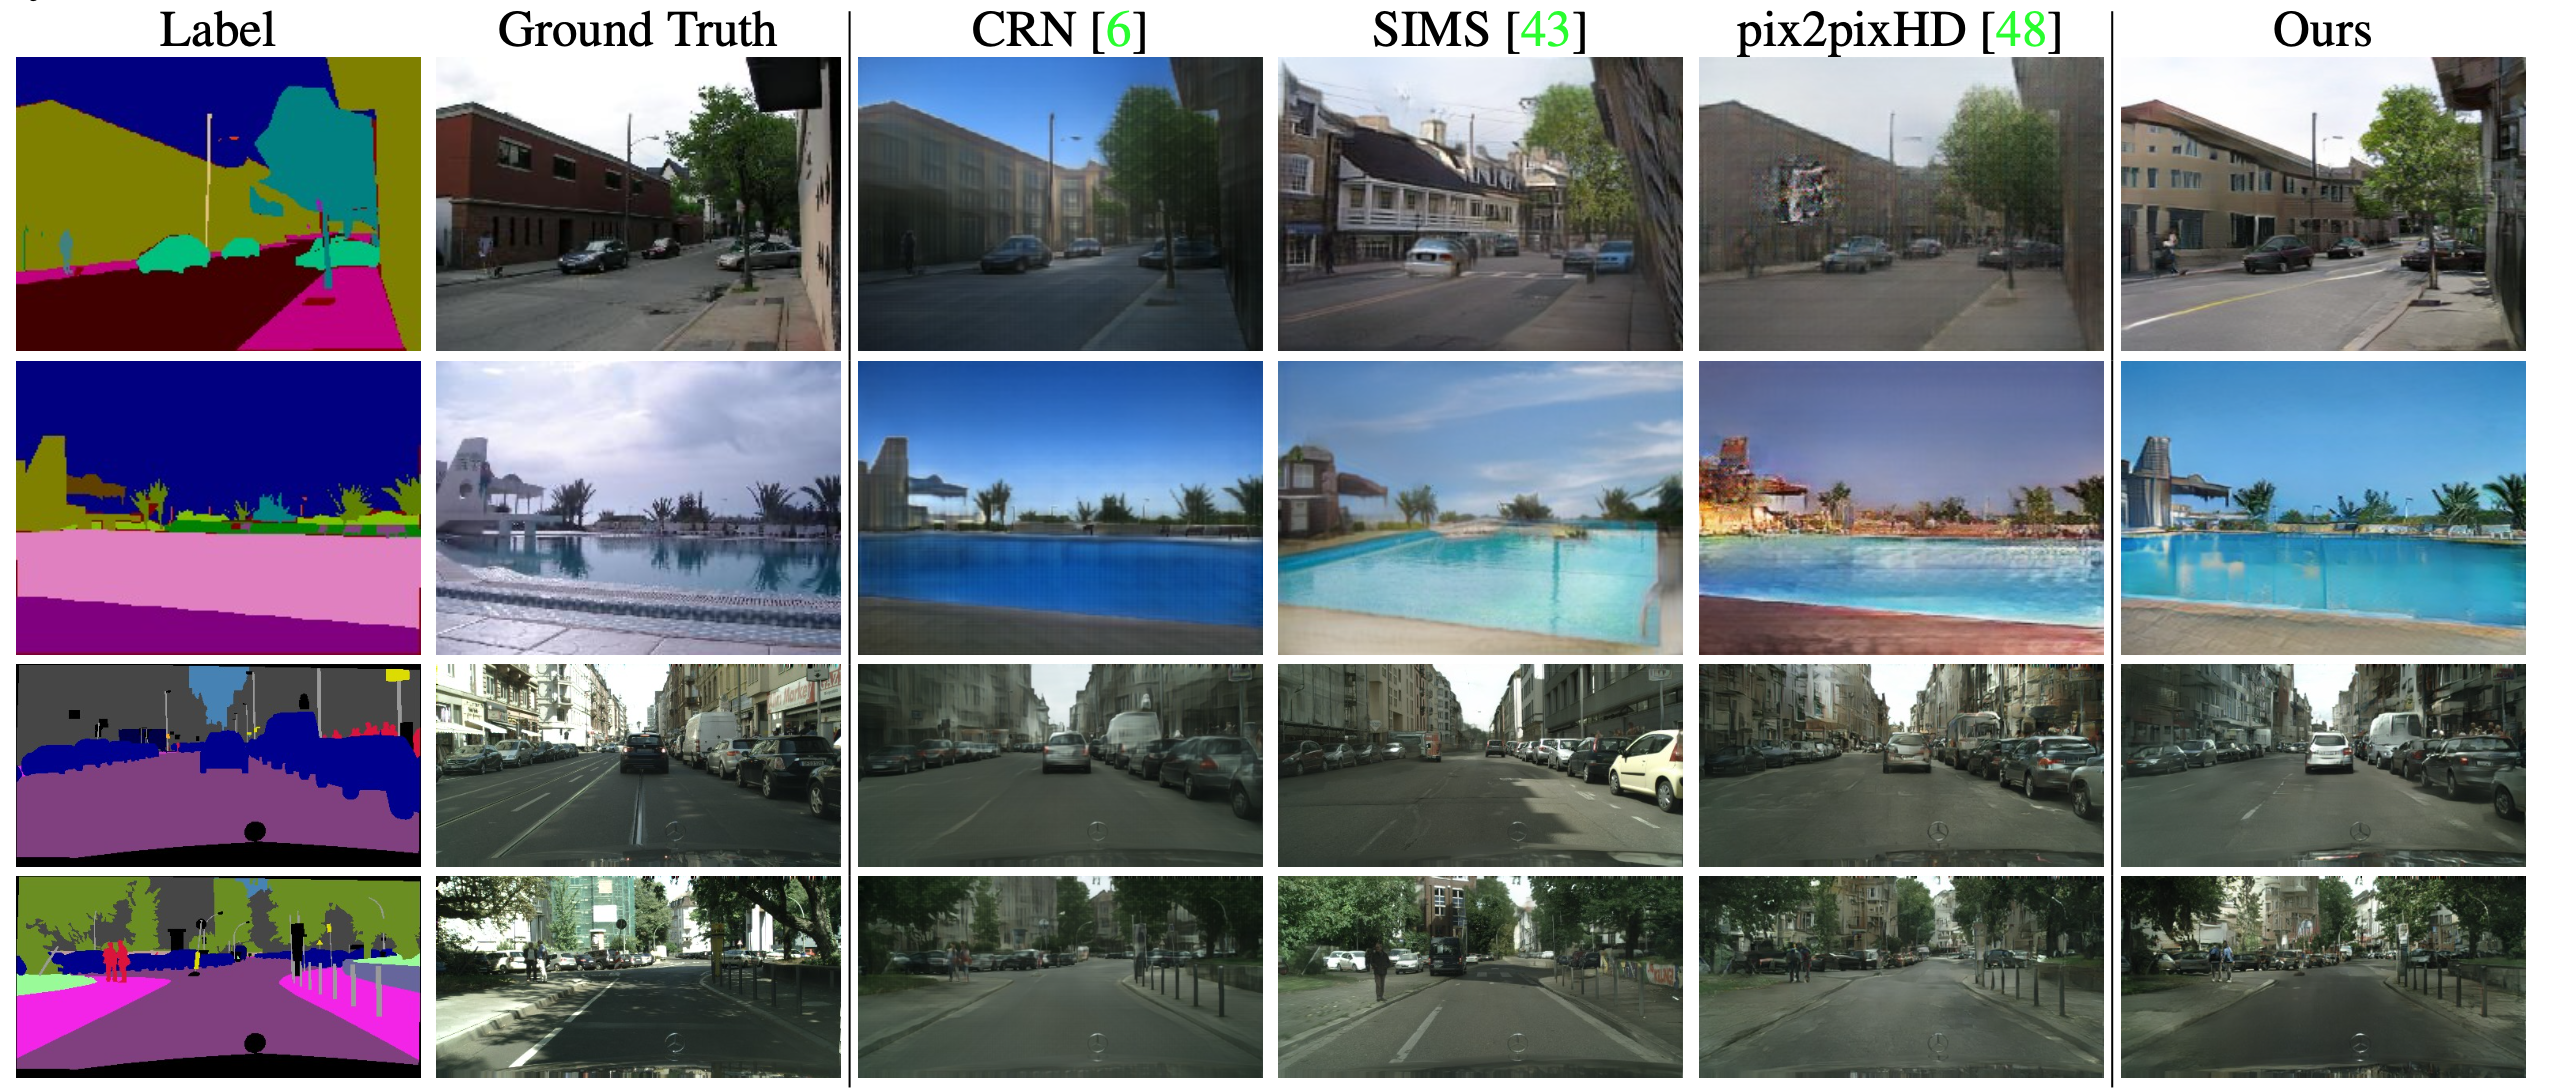
\includegraphics[width=0.9\linewidth]{figures/related_work.png} 
        \caption{Visual Comparison of Park et al. to Related Works}
    \end{figure}
\end{frame}

\begin{frame}
\frametitle{Related Work: \textbf{C}ascaded \textbf{R}efinement \textbf{N}etwork (CRN)}
    \begin{itemize}
    	\item The architecture consists of a \textbf{cascade} of refinement modules which operate at \textbf{different resolutions} each
    	\item Each layer is followed by convolutions, normalization and a non-linearity \cite{chen2017photographic}
    \end{itemize}
    \begin{figure}
        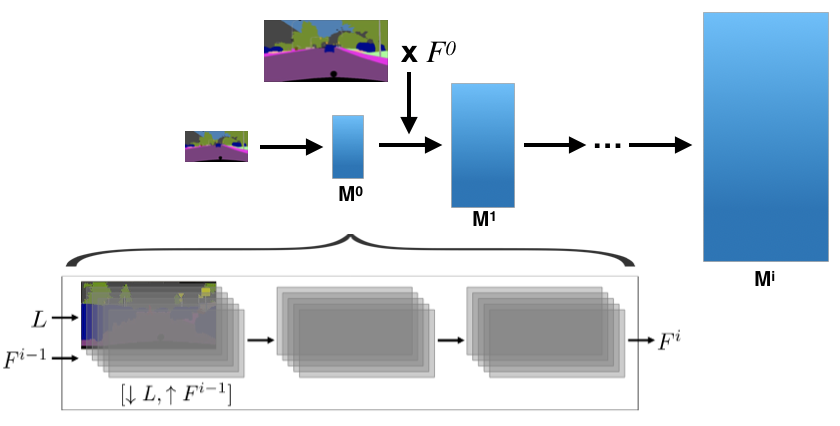
\includegraphics[scale=0.6]{figures/CRN_architecture.png}
        \caption{Network Architecture of CRN}
    \end{figure}
\end{frame}

\begin{frame}
\frametitle{Related Work: SIMS}
    \begin{itemize}
        \item SIMS = \textbf{S}emi-parametric \textbf{IM}age \textbf{S}ynthesis
    	\item Image synthesis is performed by \textbf{"stitching"} parts of images together. The parts of the images stem from a memory bank of \textbf{image segments} which is created from a training set of images beforehand
    	\cite{qi2018semi}
    \end{itemize}
    \begin{figure}
    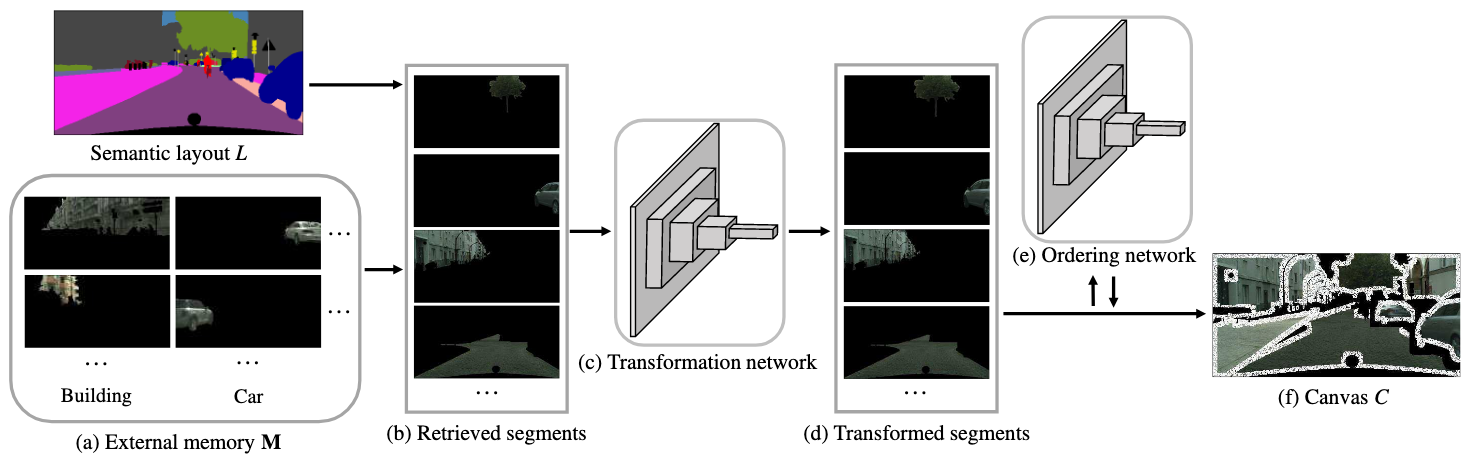
\includegraphics[scale=0.45]{figures/sims_architecture.png}
    \caption{Canvas Generator for SIMS}
    \end{figure}
\end{frame}

\begin{frame}
\frametitle{Related Work: pix2pixHD}
\begin{itemize}
	\item Focus images with \textbf{high resolution} and \textbf{photorealism}
	\item \textbf{Approach:} using a coarse-to-fine generator and multi-scale discriminator architectures
    \item Decompose the generator into two \textbf{sub-networks} \textit{G1} and \textit{G2} to combine the \textbf{global} and \textbf{local} information \cite{wang2018high}
\end{itemize}
\centering
\begin{figure}
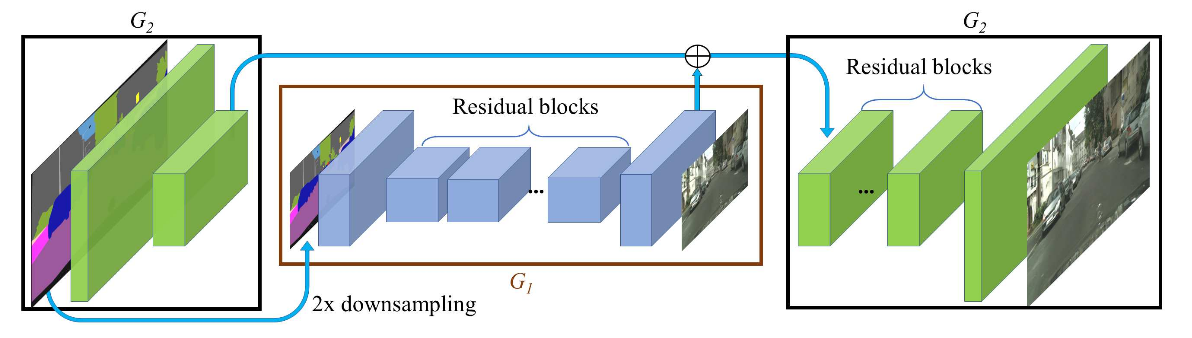
\includegraphics[scale=0.55]{figures/pix2pixHD.png} 
\caption{Network Architecture of pix2pixHD's Course-to-fine Generator}
\end{figure}
\end{frame}

\begin{frame}
\frametitle{Related Work: pix2pixHD}
\textbf{Multi-scale Discriminator}
\begin{itemize}
    \item \textbf{Problem:} Discriminator needs \textbf{large receptive field} to differentiate between \textbf{high resolution} images. However, constructing a deeper network could lead to \textbf{overfitting} and a larger \textbf{memory} footprint
    \item \textbf{Solution:} Multi-scale discriminators: decompose into 3 identical discriminators (\textit{D1}, \textit{D2}, \textit{D3}) with \textbf{different image scales}
\end{itemize}
\begin{figure}
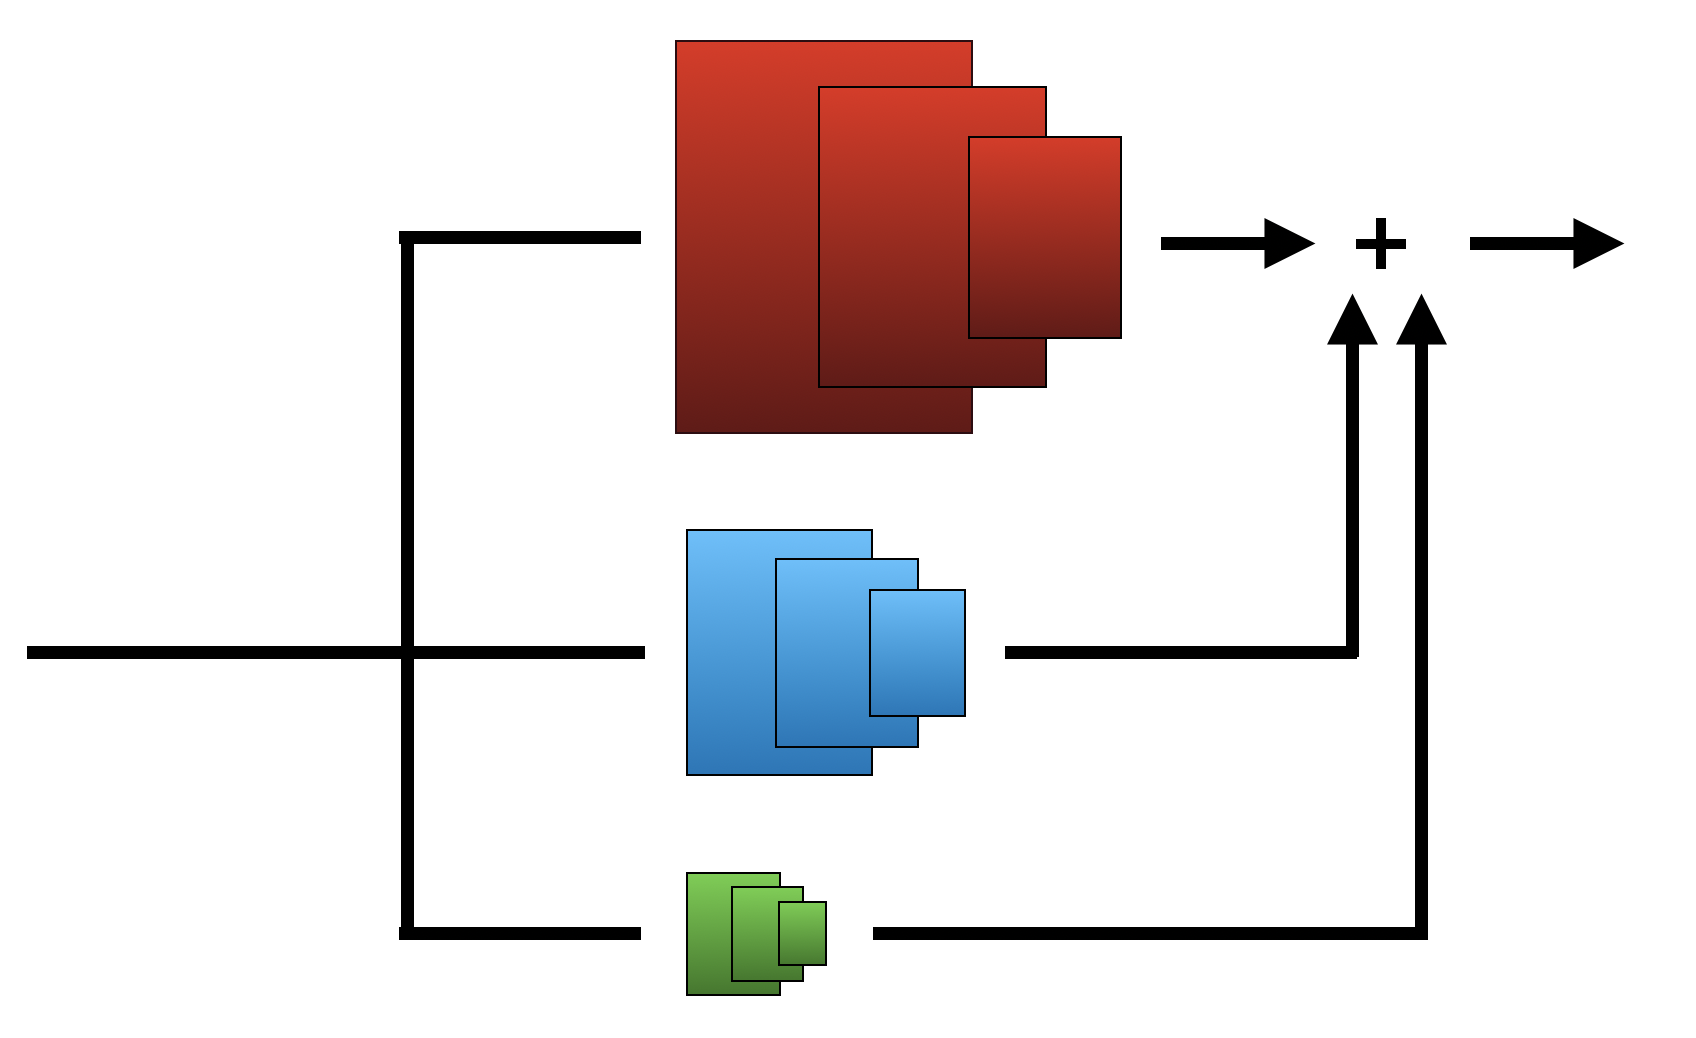
\includegraphics[scale=0.17]{figures/multi_scale_discriminator.png} 
\caption{Architecture of the \textbf{pix2pixHD's} Multi-Scale Discriminator}
\end{figure}
\end{frame}

\begin{frame}
\frametitle{Issues with Related Works}
\begin{itemize}[<+->]
	\item \textbf{Current Approach}: Semantic information is direct input to neural network and processed through stacks of convolution, normalization, and non-linearity layers
	\item \textbf{Problem}: Semantic information is not well preserved (normalization layers tend to "wash away" semantic information)
	\item \textbf{Solution}: A novel conditional normalization method (SPADE) that modulates the activations using semantic layouts
\end{itemize}
\end{frame}

% SEMANTIC IMAGE SYNTHESIS
\section{Semantic Image Synthesis}
\frame{\frametitle{Outline}\tableofcontents[currentsection]}

\begin{frame}{Spatially-Adaptive Denormalization (SPADE) Layer}
    
        \begin{minipage}[t]{0.5\linewidth}
            \begin{figure}
                \centering
                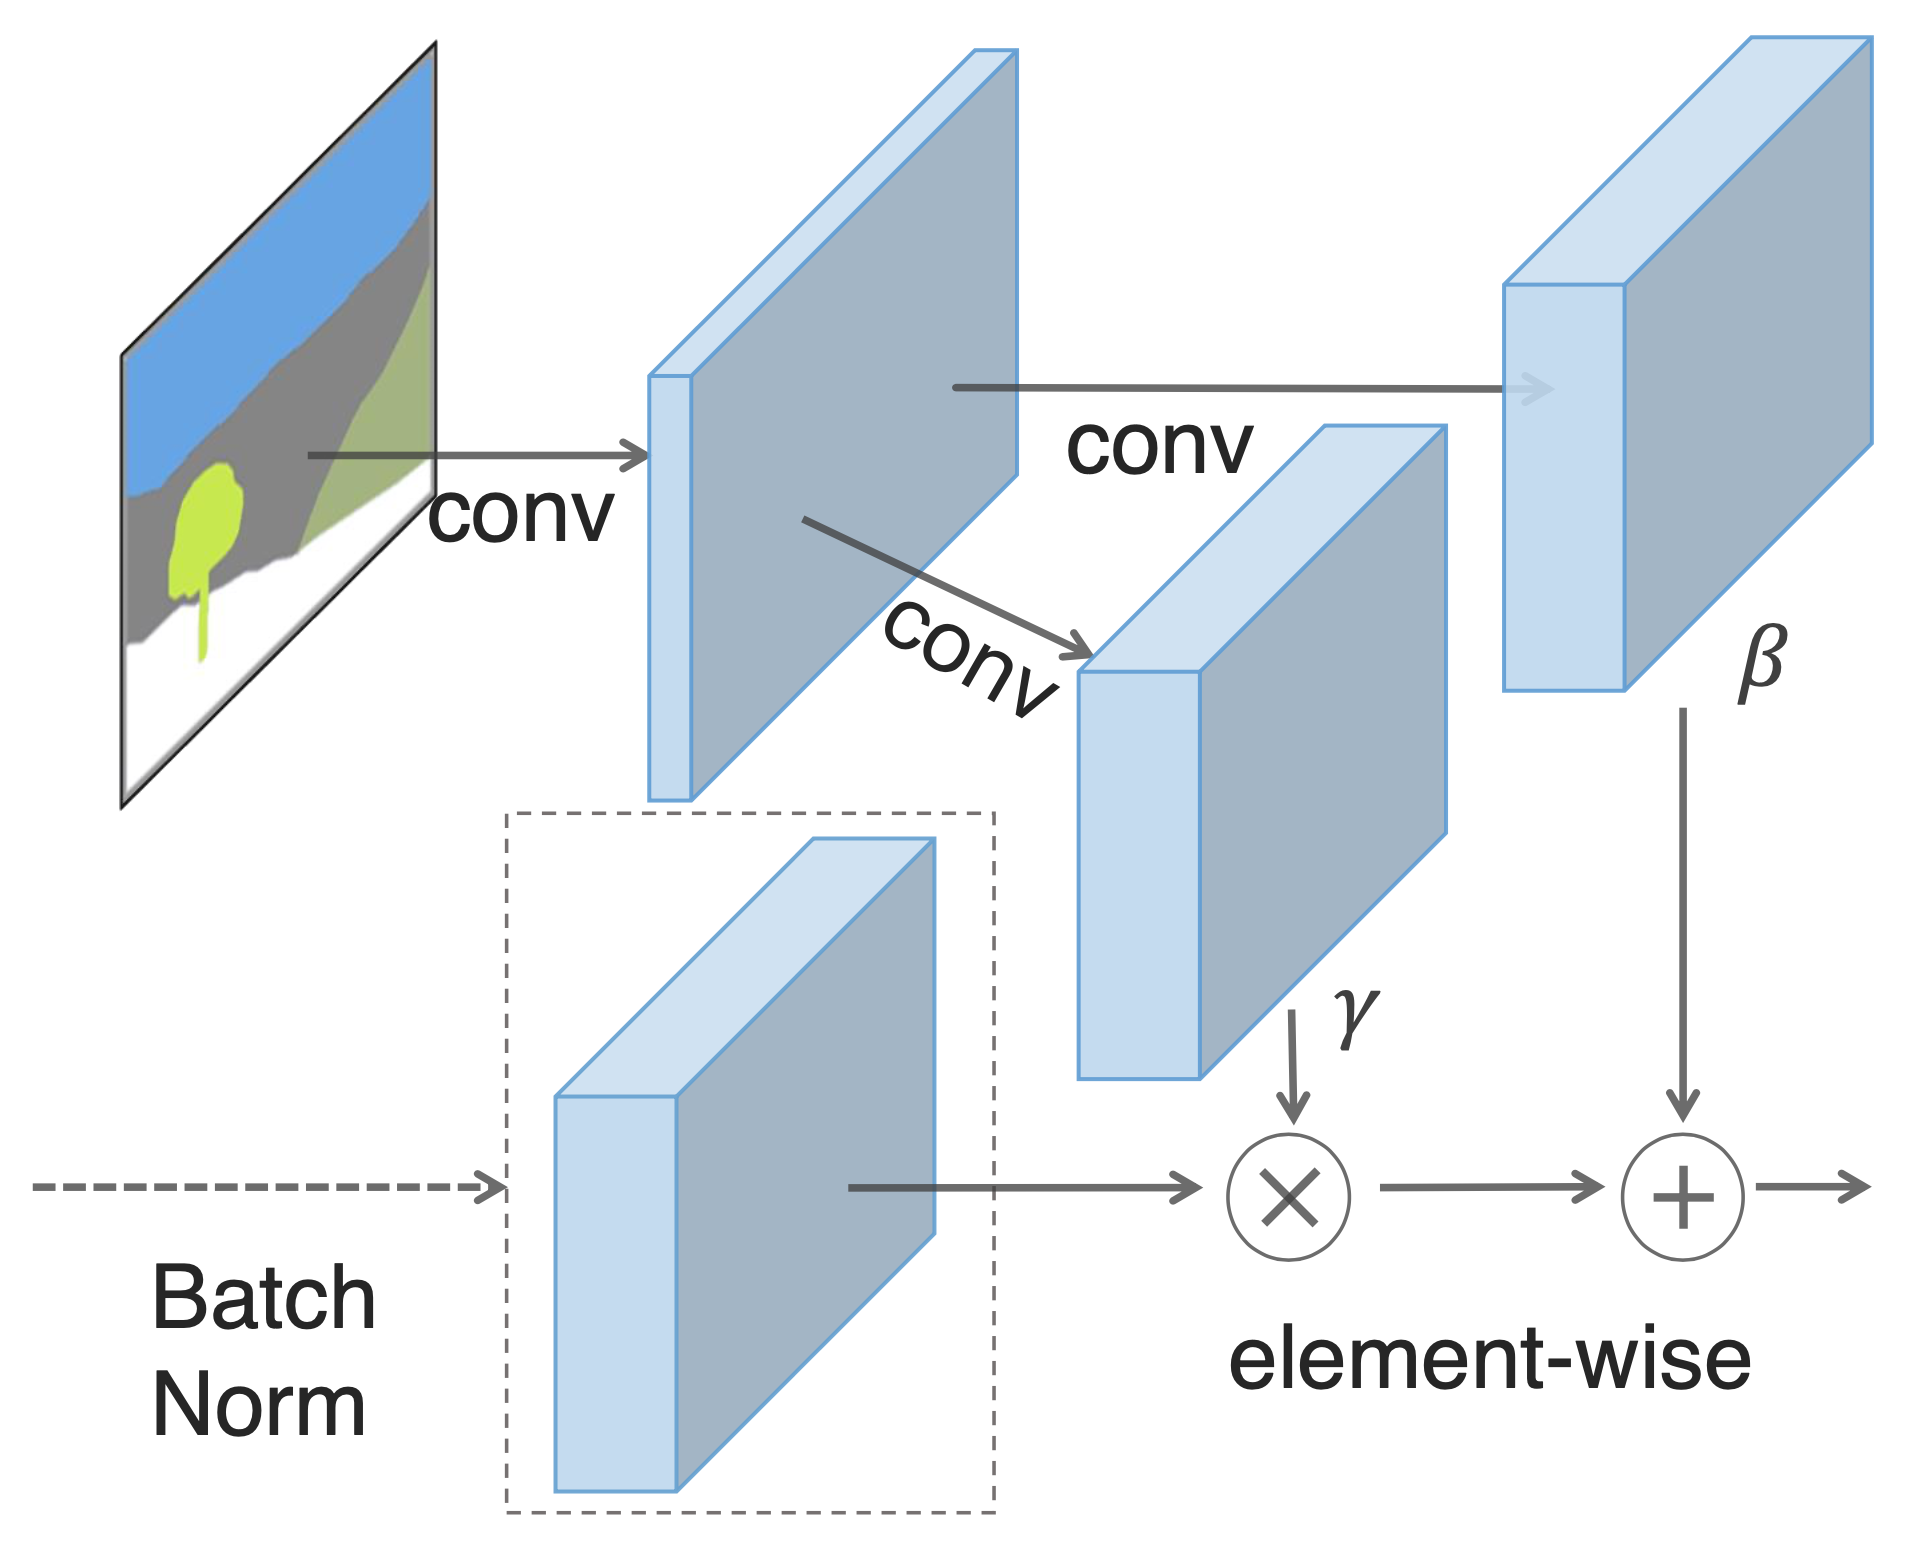
\includegraphics[width=0.9\textwidth]{figures/spade.png}
                \caption{The novel SPADE Layer}
            \end{figure}
        \end{minipage}
        \hspace{0.5cm}
        \begin{minipage}[t]{0.4\linewidth}
            \vspace{1cm} \begin{enumerate}
                \item Unconditional normalization of activations of previous layer with BatchNorm
                \item Denormalization with modulation parameters (scale $\gamma$ and bias $\beta$)
            \end{enumerate}
            \vfill 
            
        \end{minipage}
    
    \pause
    \begin{block}{Novelty}
        \begin{itemize}
            \item $\gamma$ and $\beta$ are learned and depend on location in segmentation mask!
            \item Modulation parameters encode semantic layout 
        \end{itemize}
    \end{block}
\end{frame}

%NOTE: $\gamma$ and $\beta$ are not vectors, but tensors with spatial dimensions. 
%NOTE: $\gamma$ and $\beta$ are implemented with a two-layer CNN
%NOTE:  SPADE is a generalization of several existing normalization layers
% NOTE: Segmentation Mask itself is not normalized but only modulated, hence does not loose semantic information

\begin{frame}{SPADE Generator}
    \begin{figure}
        \begin{minipage}[b]{0.25\linewidth}
            \centering
            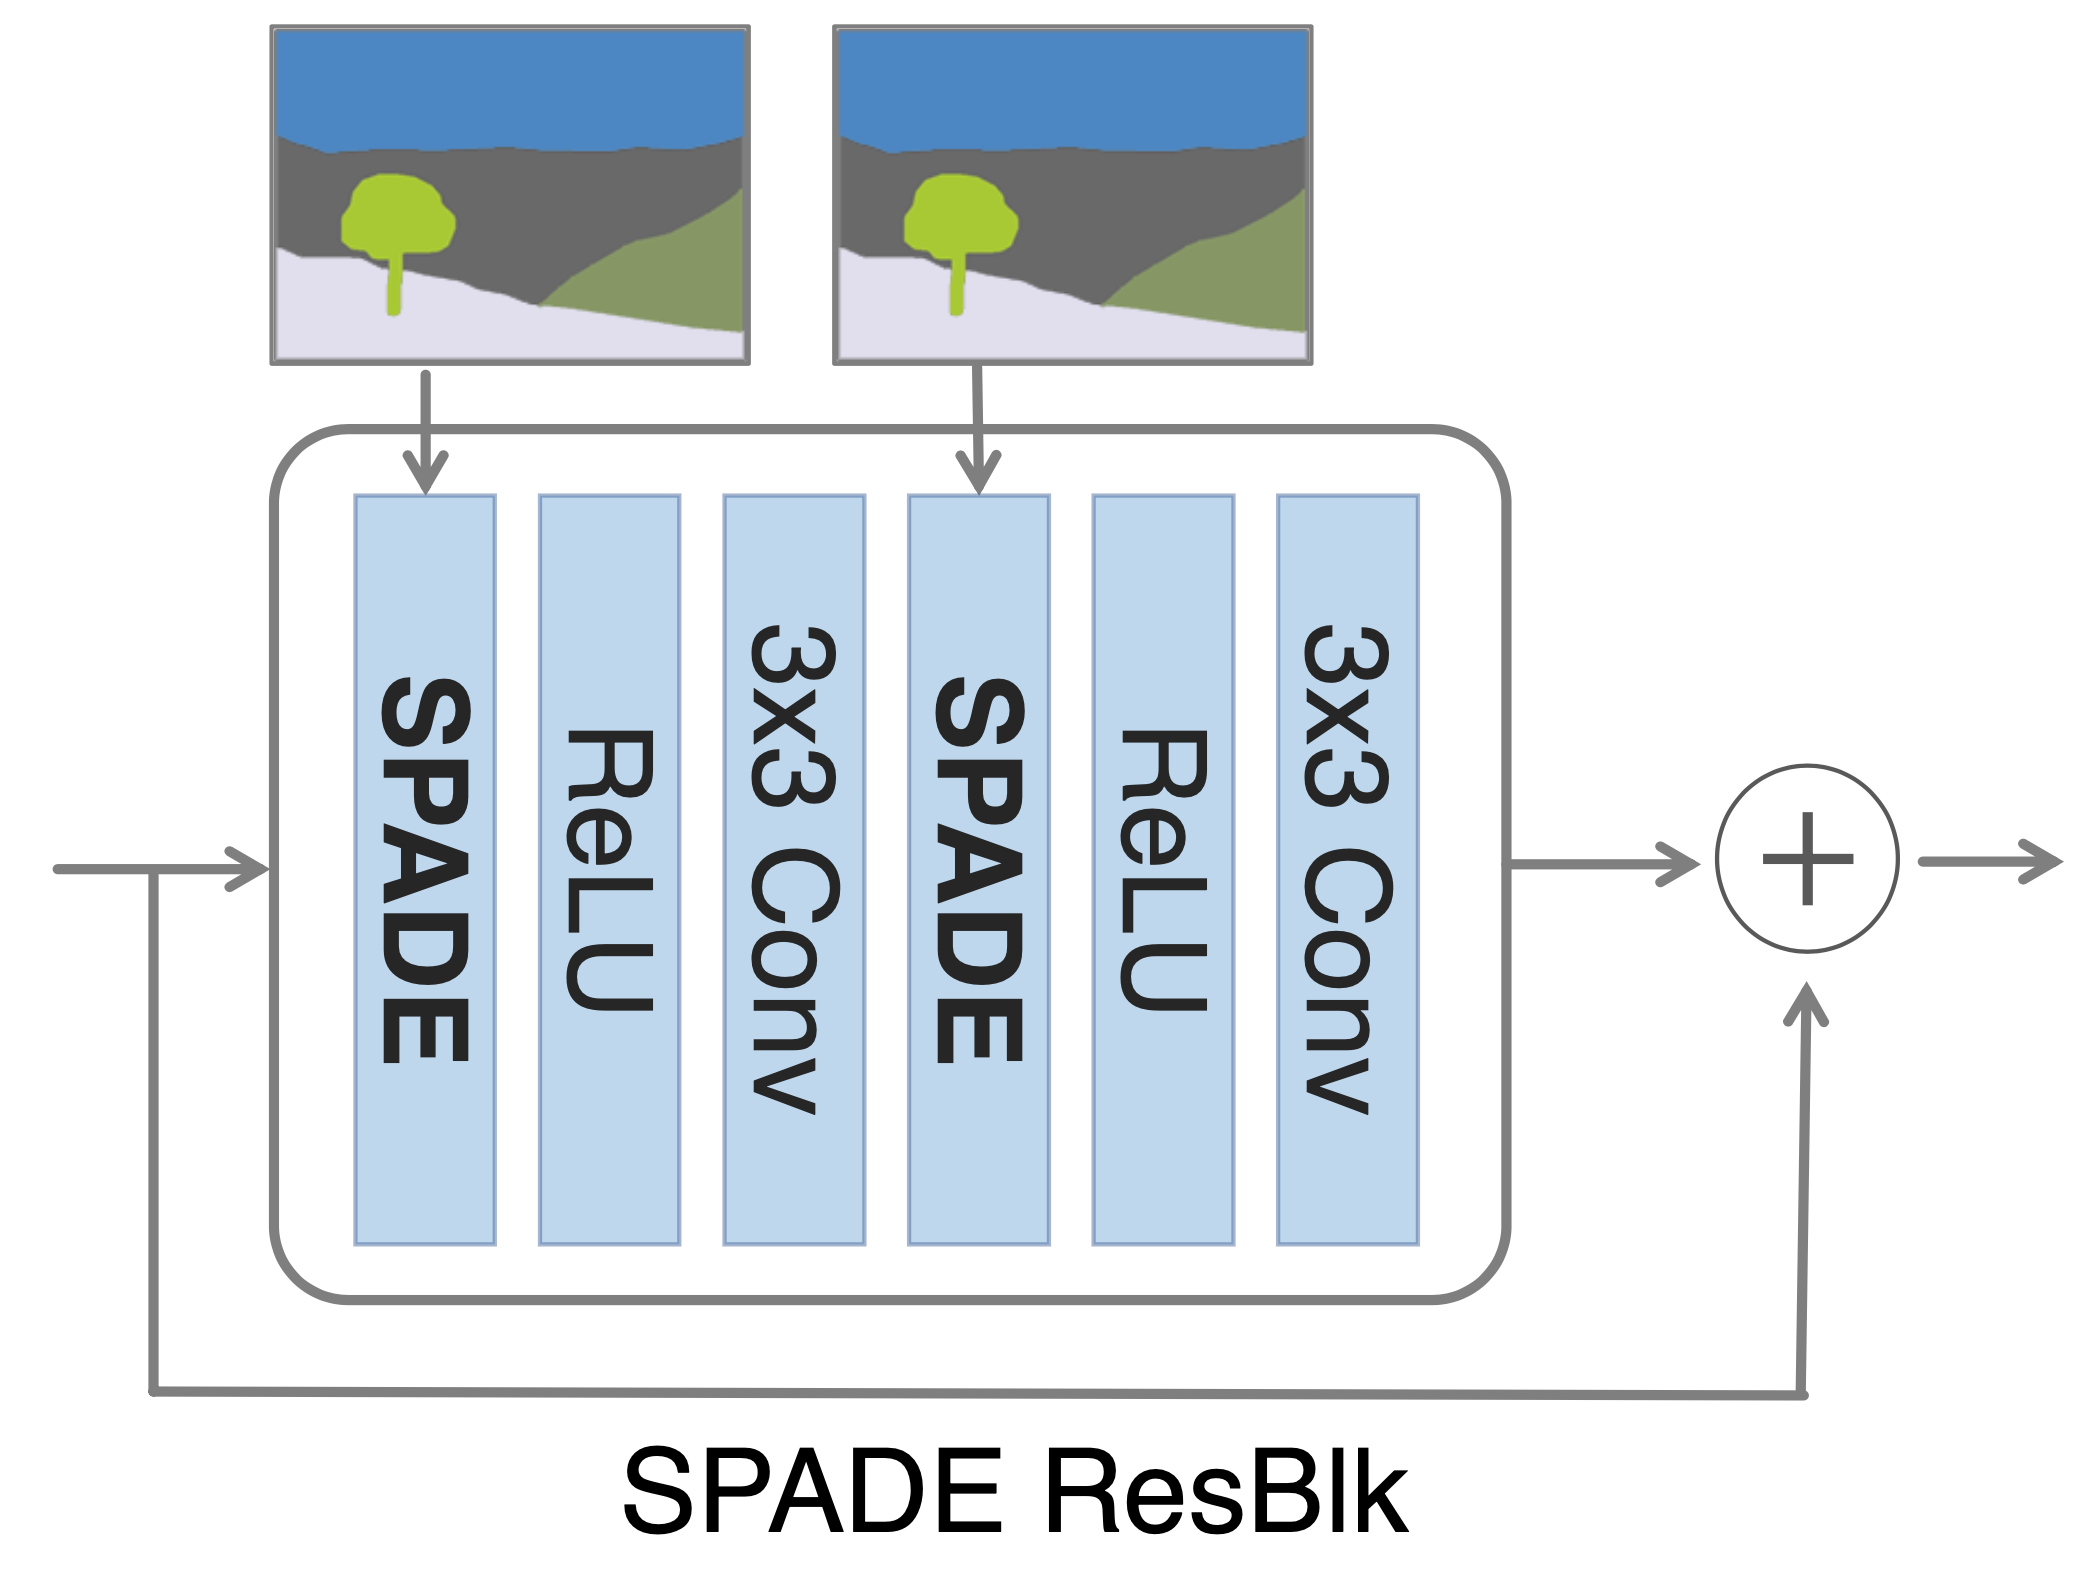
\includegraphics[width=\textwidth]{figures/spade_resblk.png}
            \caption{ResBlk}
        \end{minipage}
        \hspace{0.5cm}
        \begin{minipage}[b]{0.6\linewidth}
            \centering
            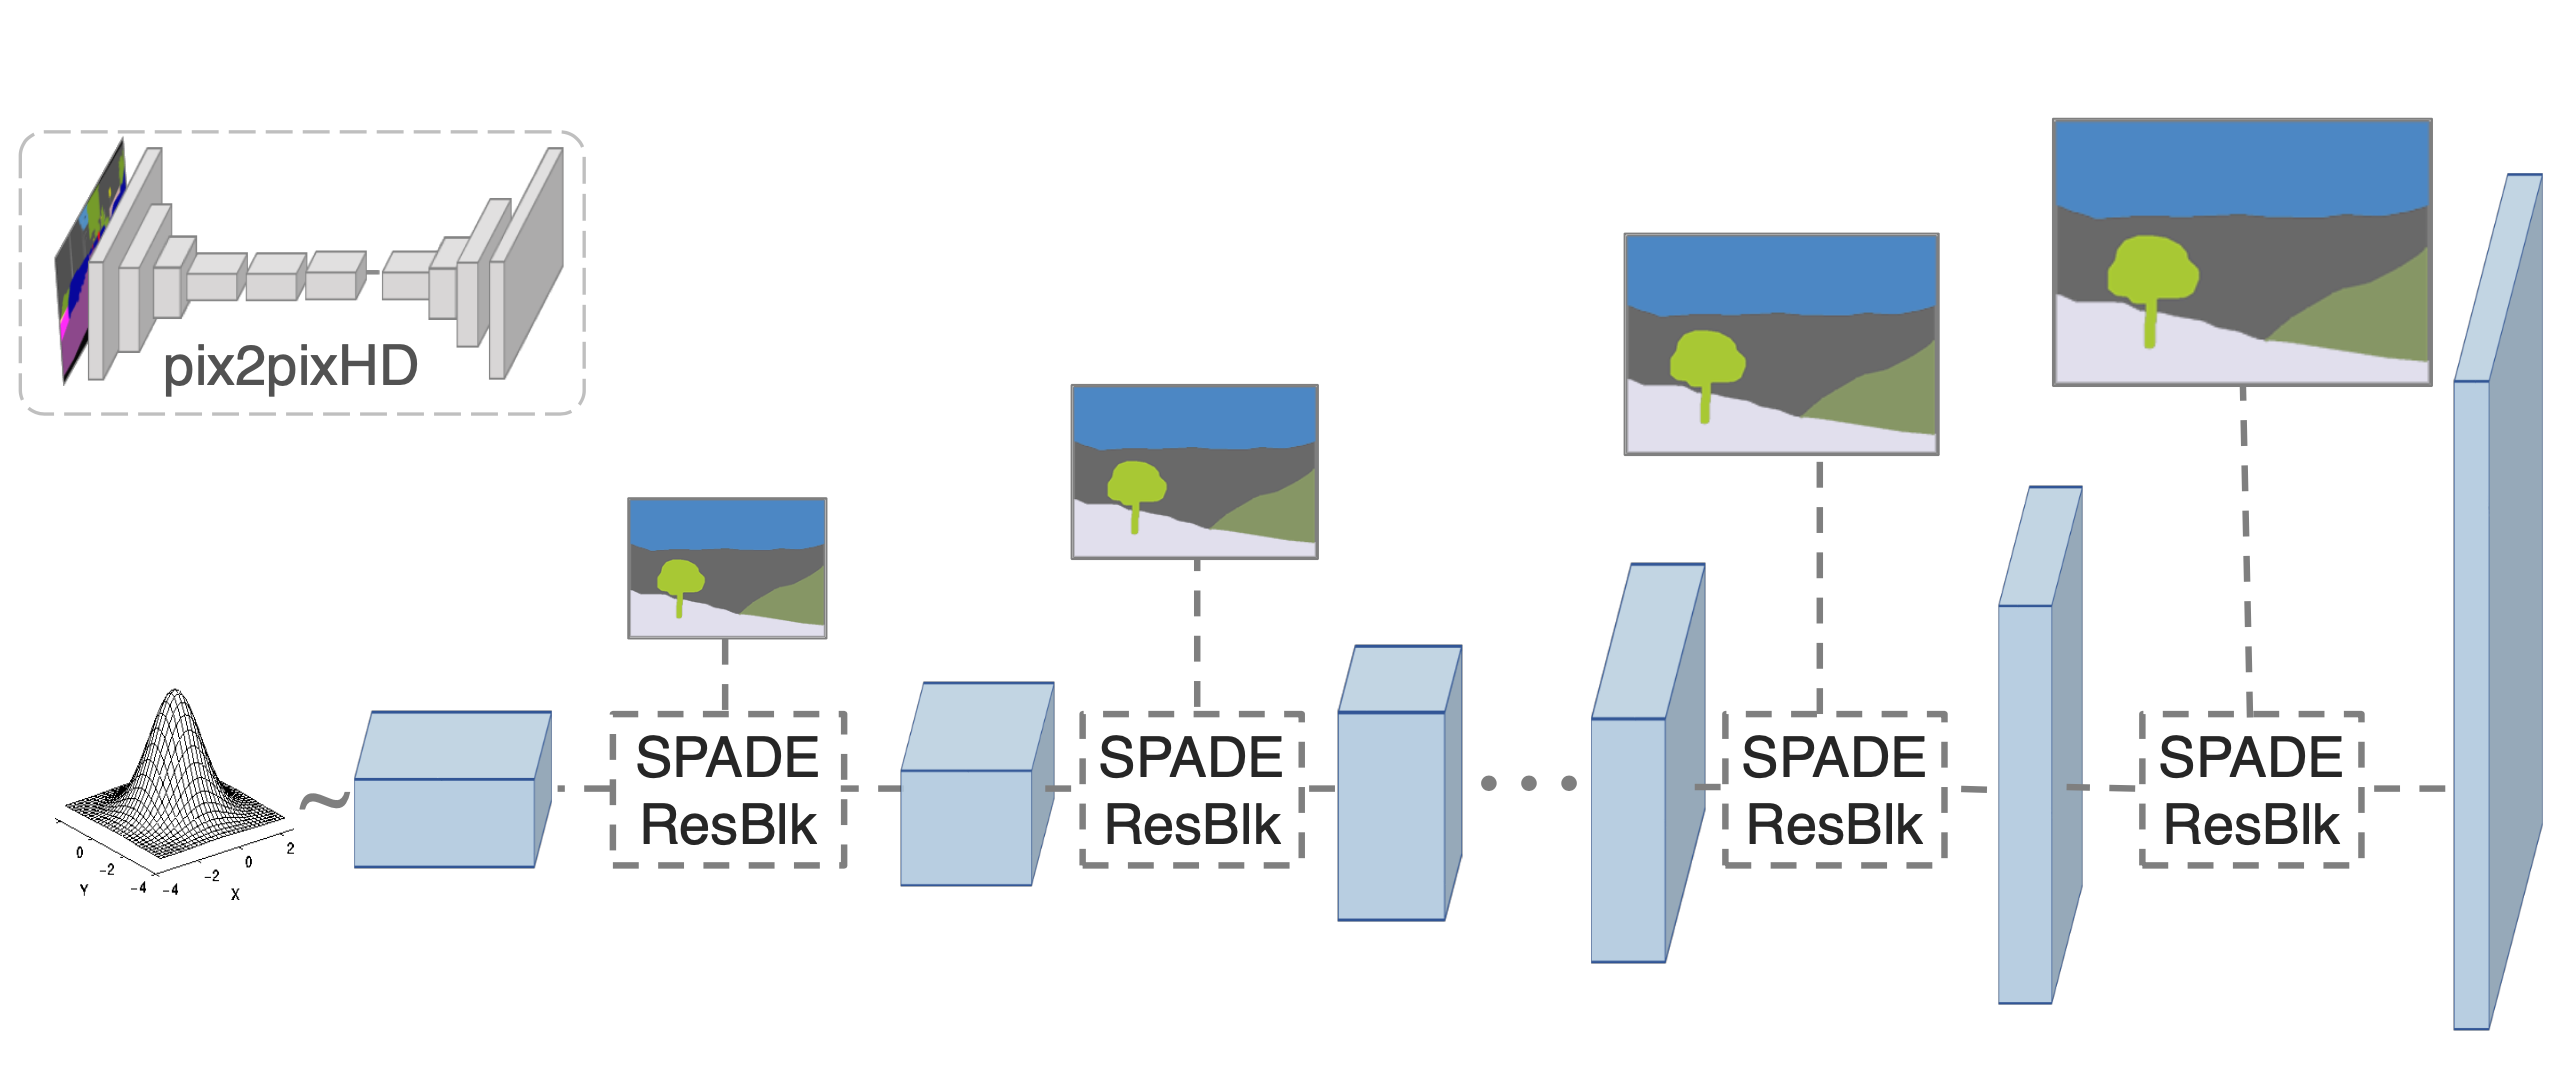
\includegraphics[width=\textwidth]{figures/spade_generator.png}
            \caption{SPADE Generator}
        \end{minipage}
    \end{figure}
    
    \begin{itemize}[<+->]
        \item ResBlk: residual block with skip connection
        \item Resized seg. masks influence generation through SPADE ResBlks
        \item Nearest neighbor upsampling
        \item Random noise fed to first layer instead of segmentation mask
    \end{itemize}
\end{frame}
% NOTE: "We use semantic maps in different scales, which enables coarse-to-fine generation"

\begin{frame}{Multi-Modal Synthesis}

\begin{figure}
    \centering
    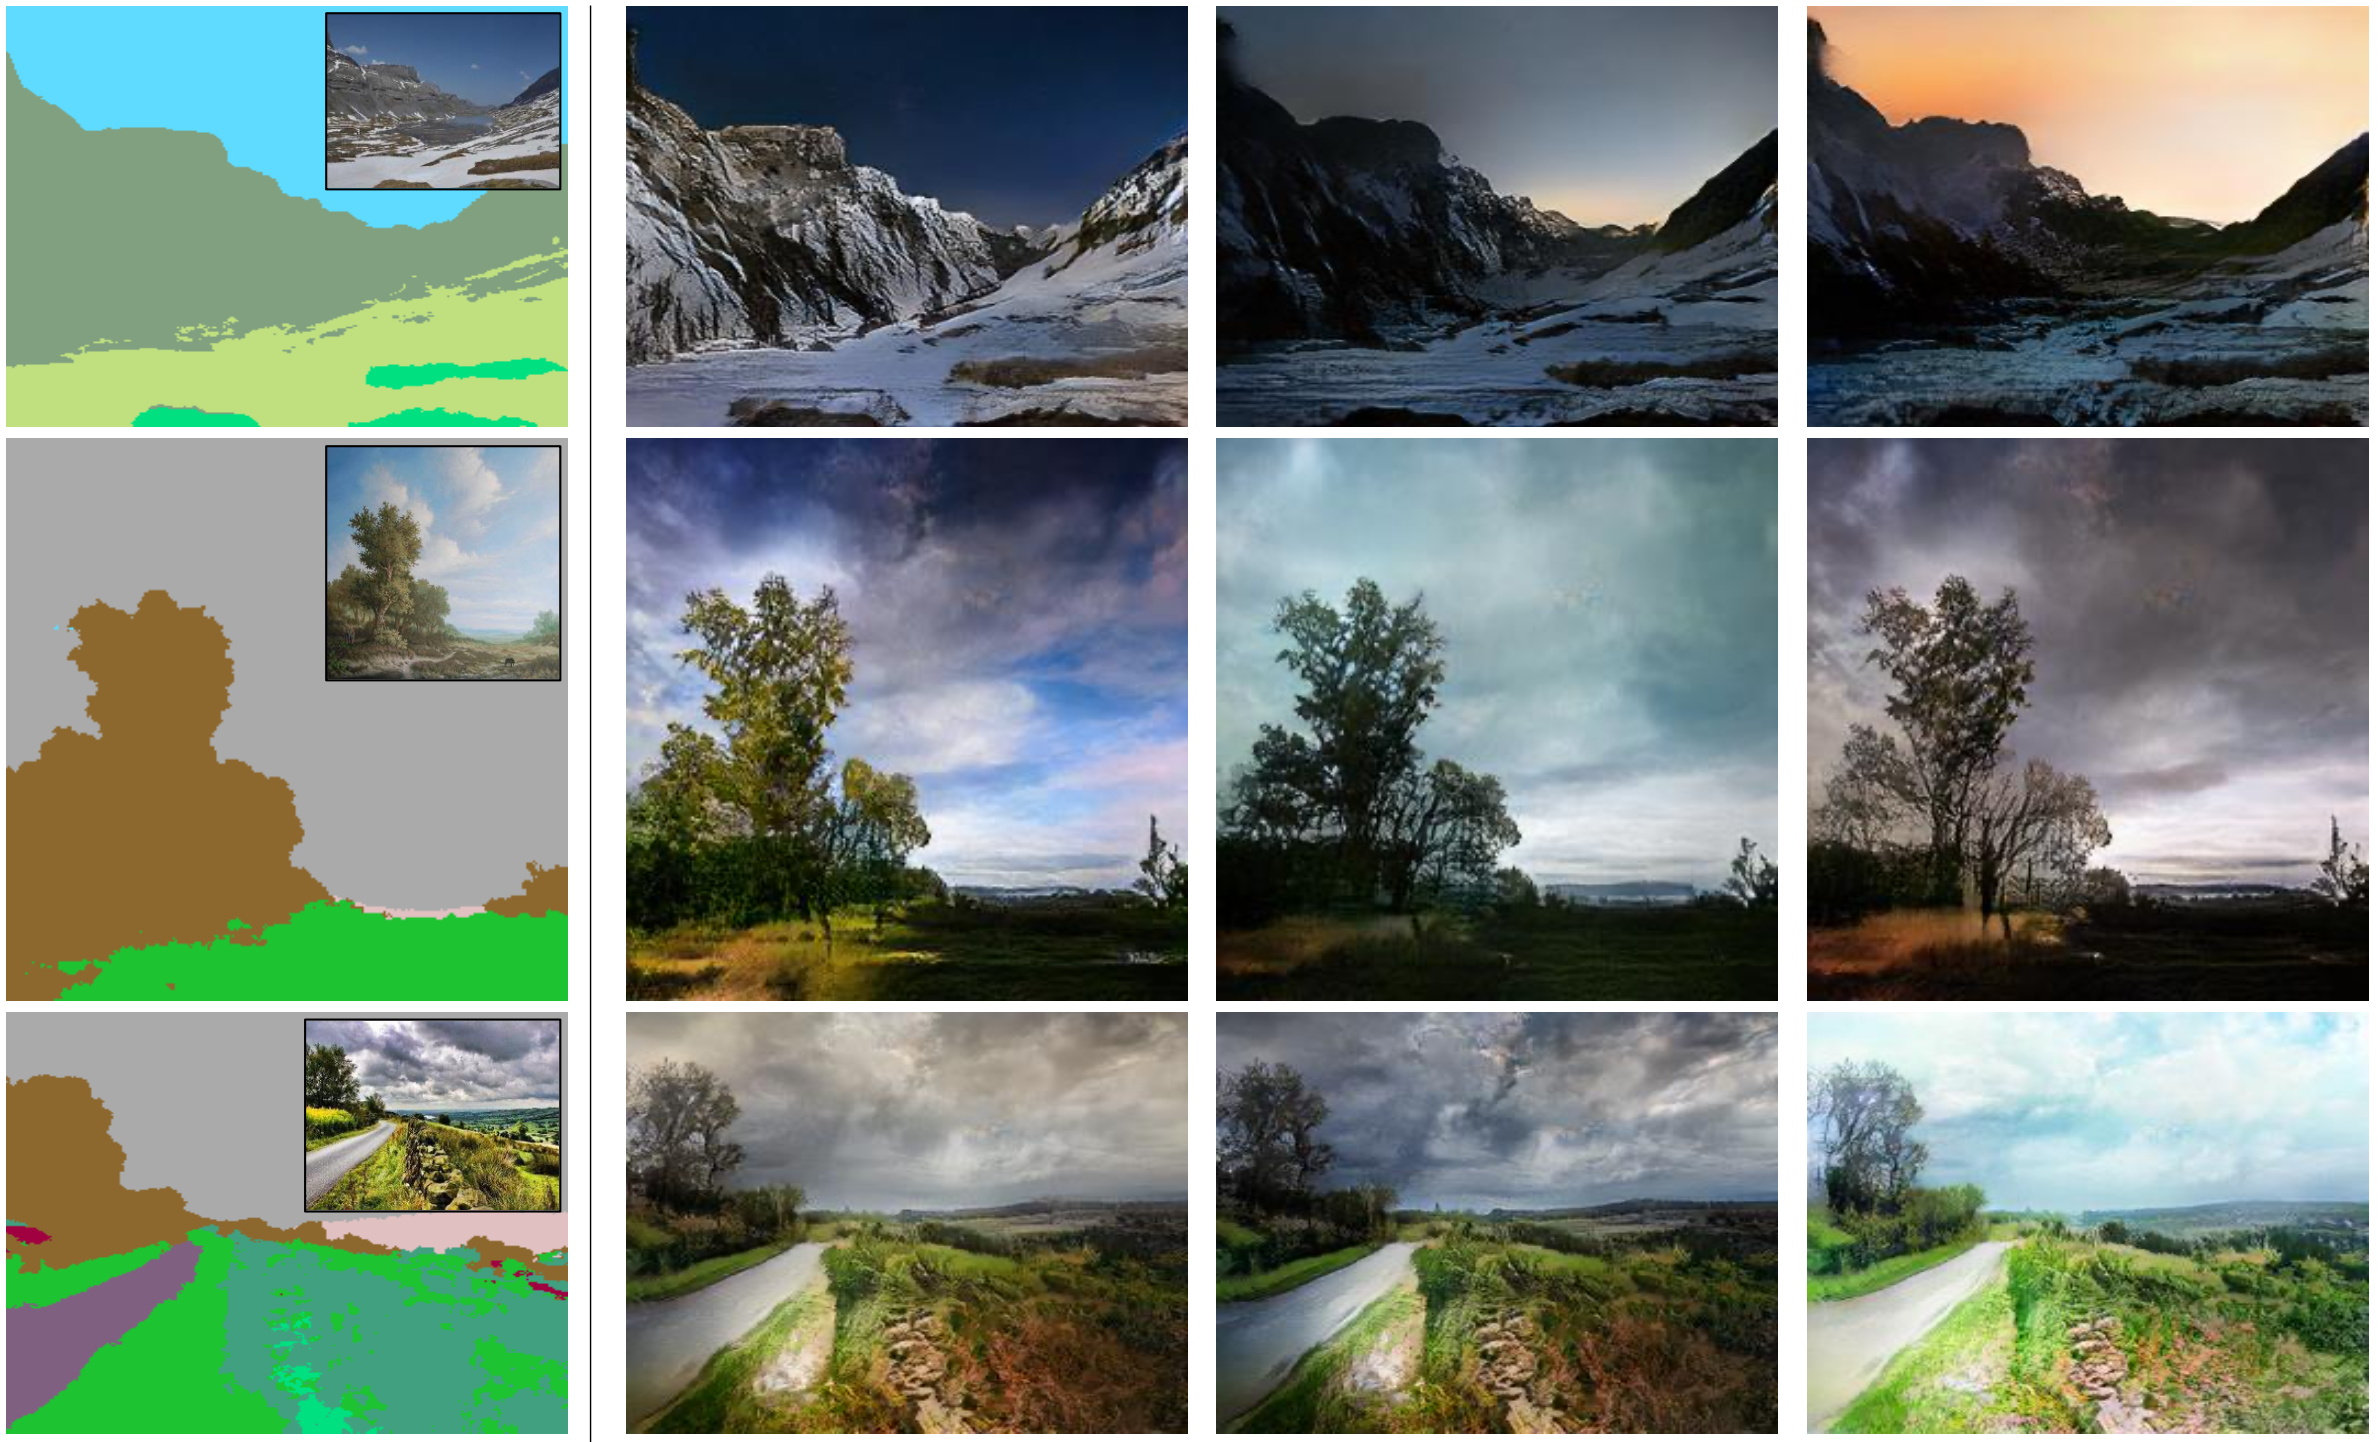
\includegraphics[width=0.8\linewidth]{figures/multi_modal.png}
\end{figure}

\begin{itemize}
    \item Different random inputs with the same segmentation mask lead to different appearances but same semantic layout 
\end{itemize}

\end{frame}

\begin{frame}{Guided Image Synthesis}

\begin{figure}
    \centering
    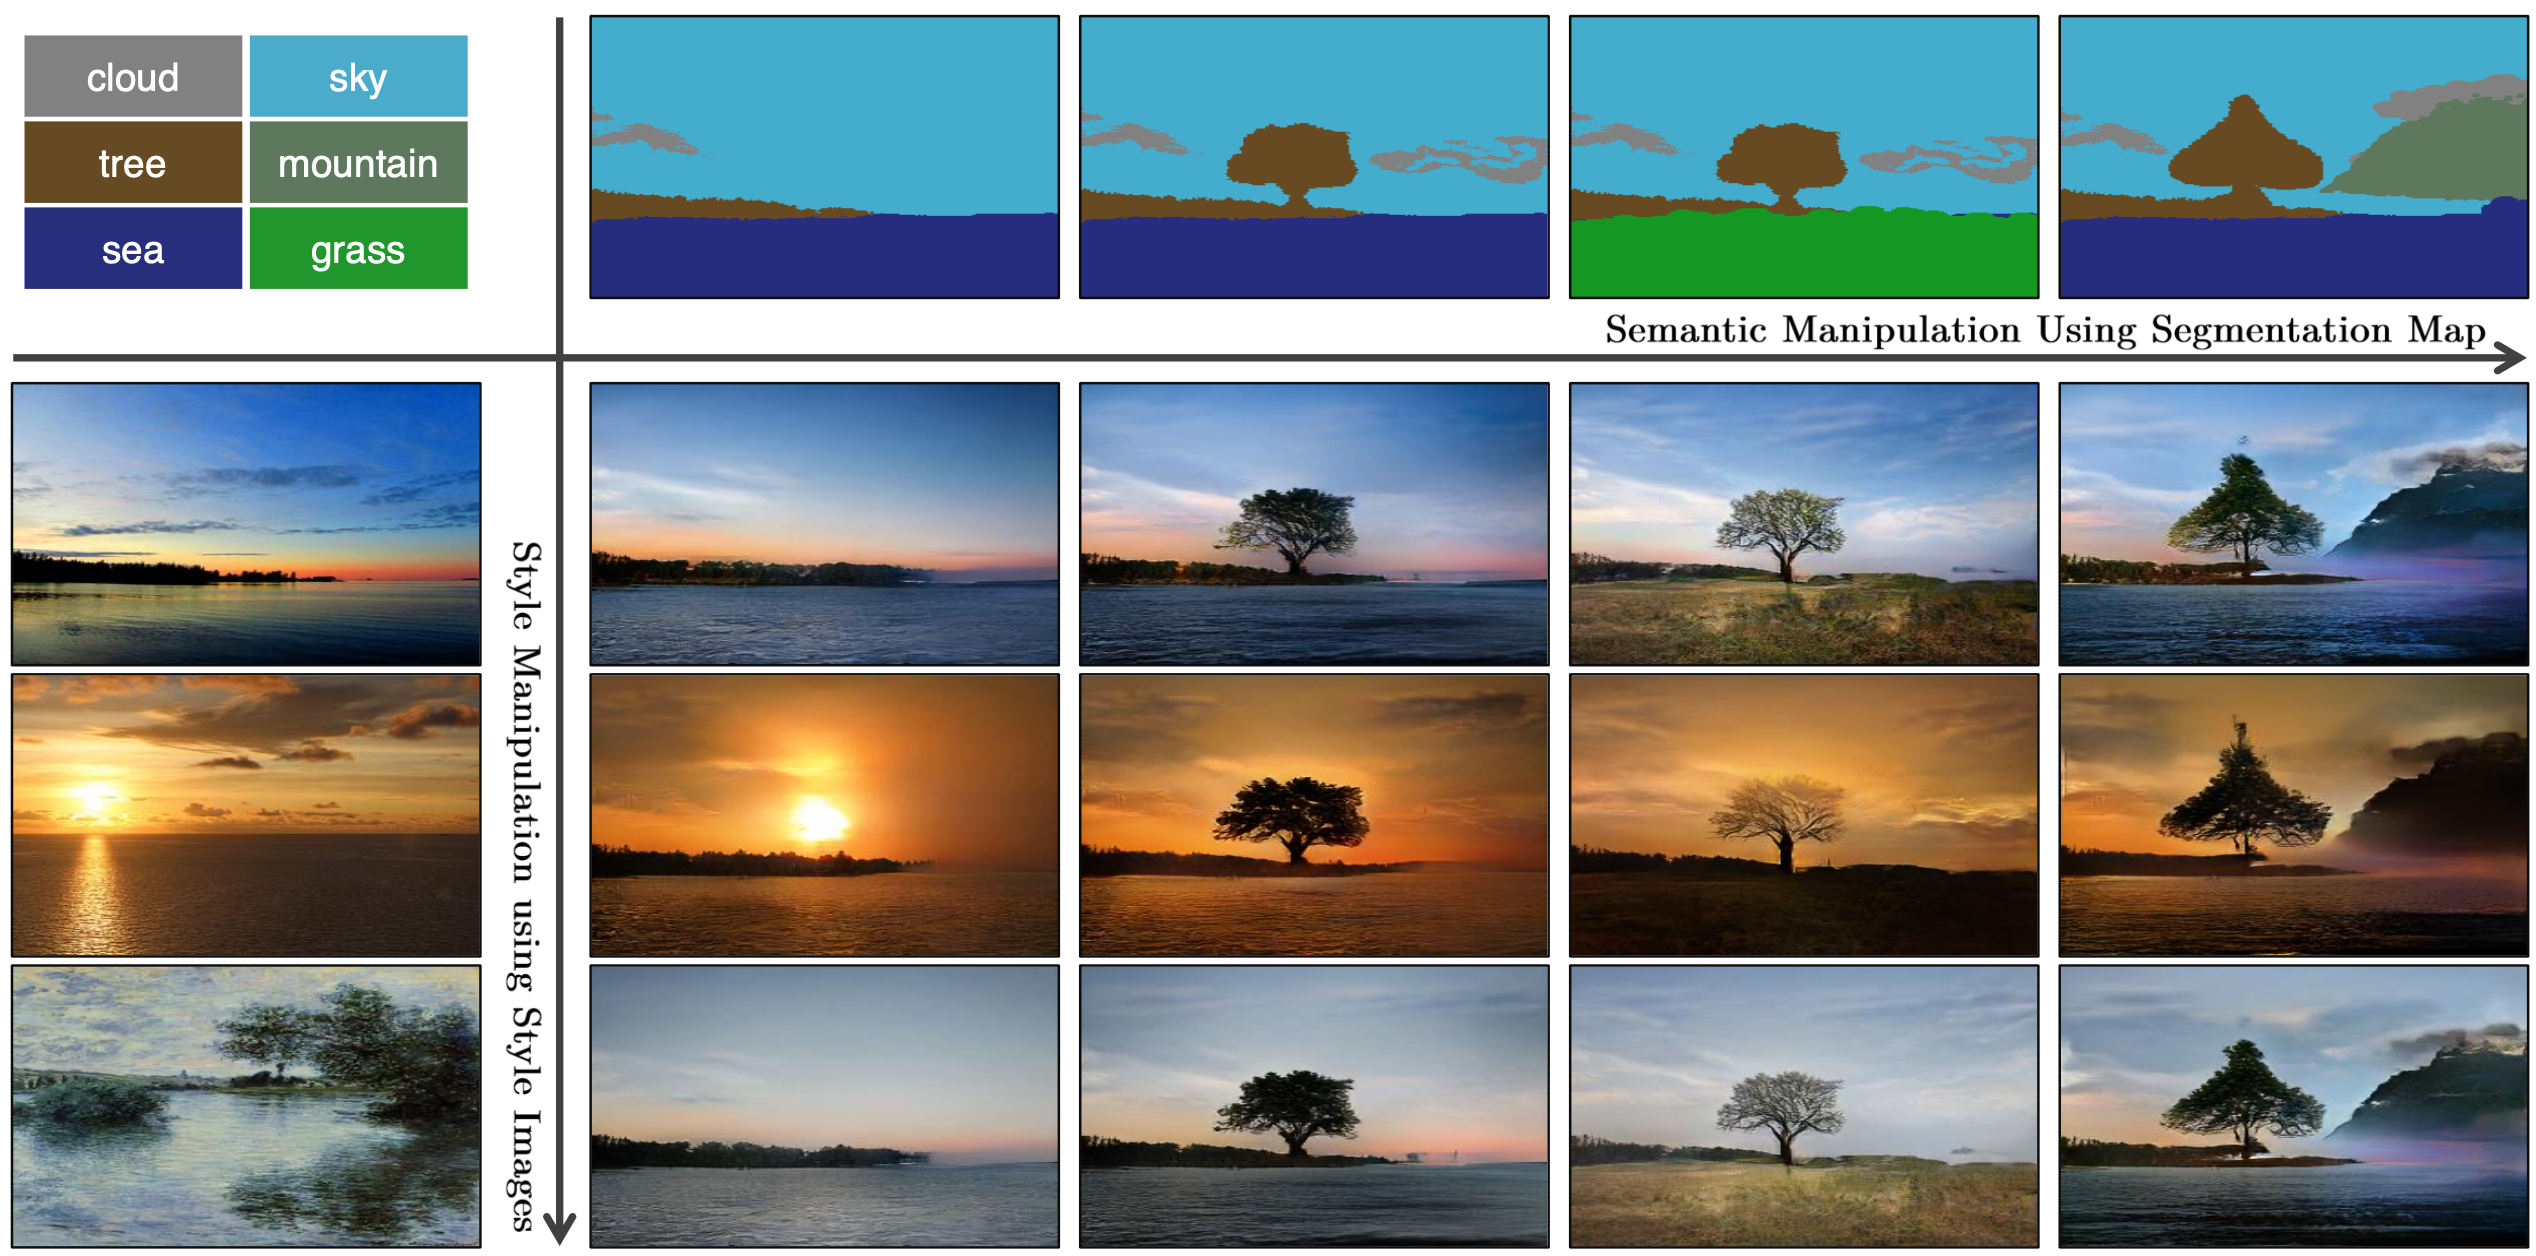
\includegraphics[width=0.8\linewidth]{figures/guided_image_syn.png}
\end{figure}

\begin{itemize}
    \item Control semantics with segmentation mask and appearance with style image (style and semantics disentanglement)
    \item Interactive web application \href{https://www.nvidia.com/en-us/research/ai-playground/}{\color{blue}{\underline{GauGAN}}}
\end{itemize}

\end{frame}

\begin{frame}{Network Architecture}

    \begin{minipage}[b]{0.3\linewidth}
        \centering
        \begin{figure}
            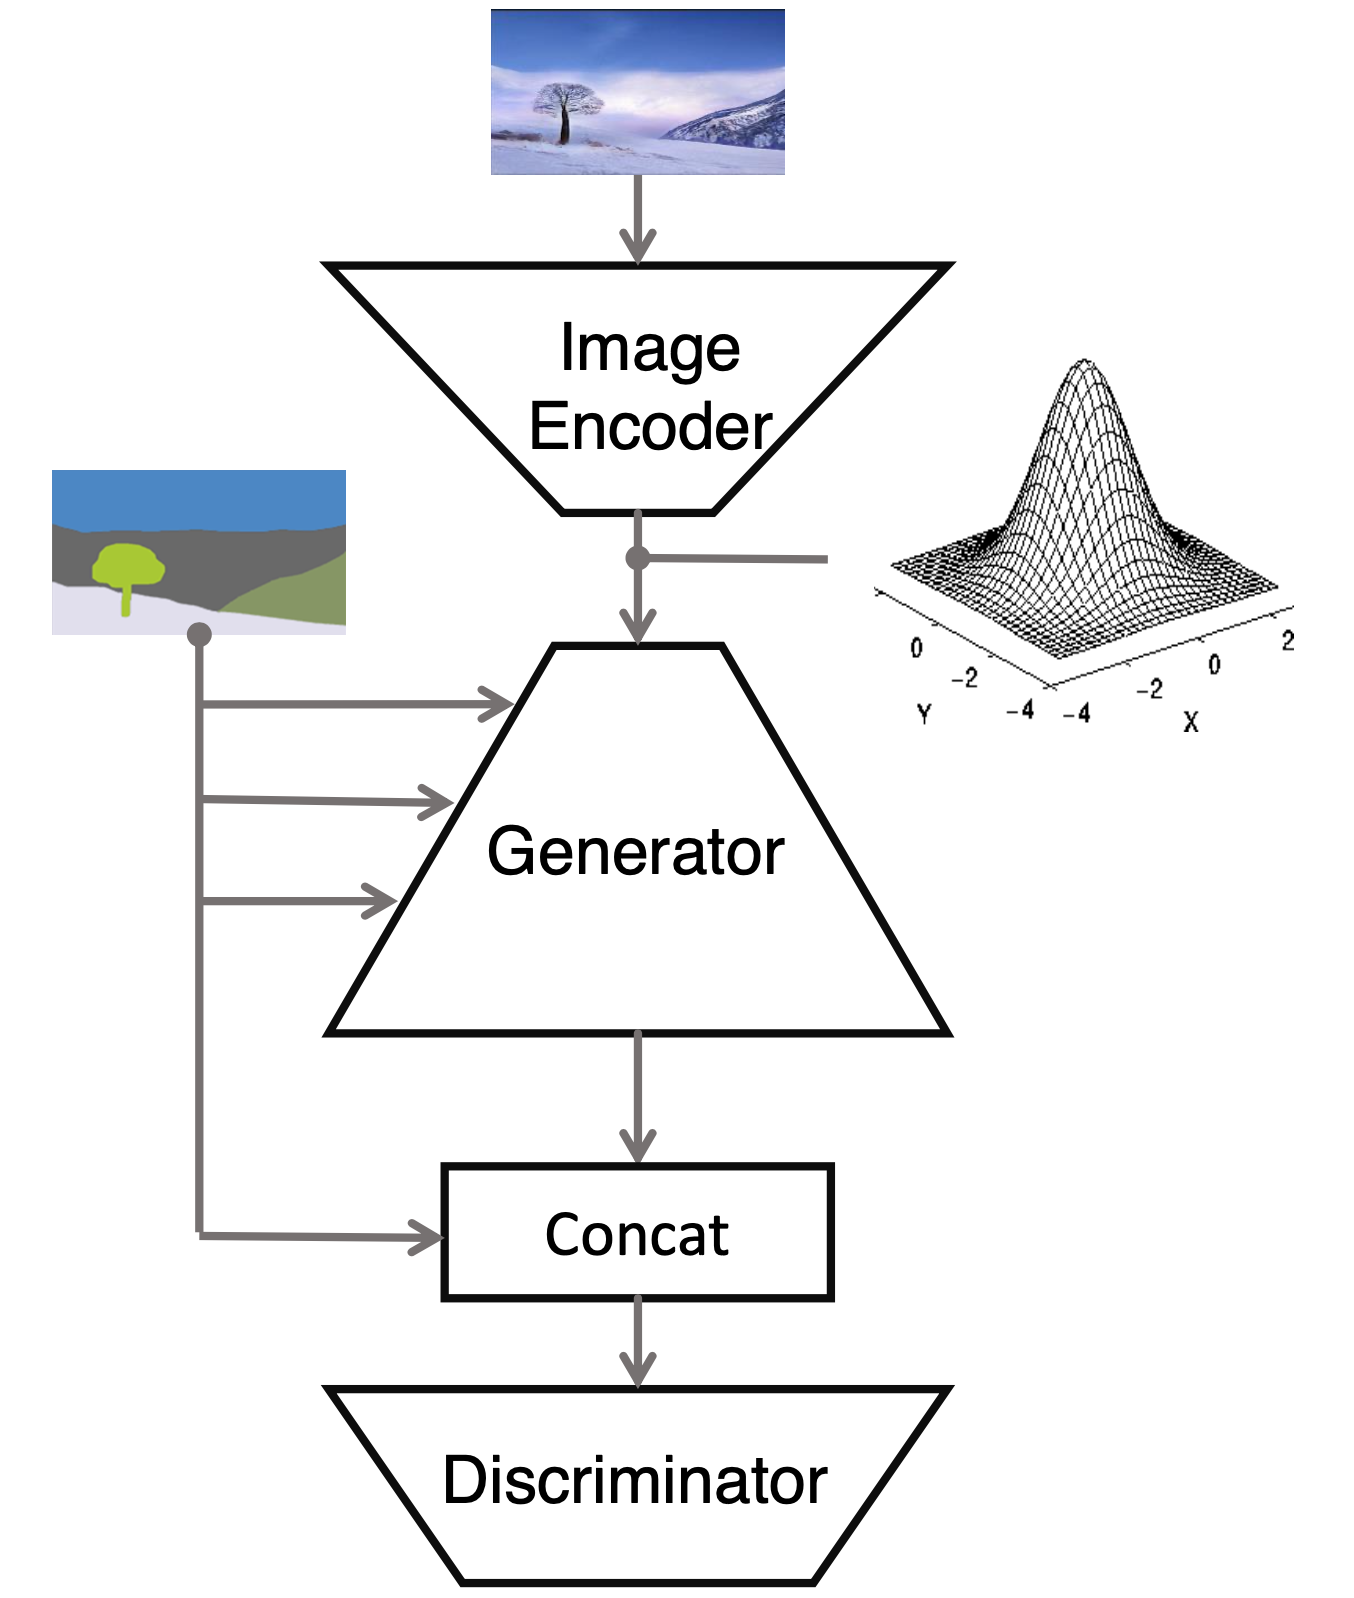
\includegraphics[scale=0.18]{figures/gan_architecture.png}
        \end{figure}
    \end{minipage}
    \hspace{0.5cm}
    \begin{minipage}[b]{0.6\linewidth}
        \centering
        \begin{itemize}[<+->]
            \item \textbf{Image encoder} captures style of a real image in a latent representation. Outputs a mean vector $\mu$ and a variance vector $\sigma^2$
            \item \textbf{Generator} combines encoded style and seg. mask to reconstruct original image (Encoder + Generator = VAE) 
            \item \textbf{Concat} concatenates segmentation mask and generated image for comparison
            \item \textbf{Discriminator} same architecture and learning objective as pix2pixHD, but replace LS-GAN loss with Hinge loss.
        \end{itemize}
    \end{minipage}
\end{frame}
% NOTE: The encoder also serves as a style guidance network at test time to capture the style of target images

% EXPERIMENTS
\section{Experiments}
\frame{\frametitle{Outline}\tableofcontents[currentsection]}
\begin{frame}{Main Datasets}
    \begin{figure}
        \begin{minipage}[b]{0.26\linewidth}
            \centering
            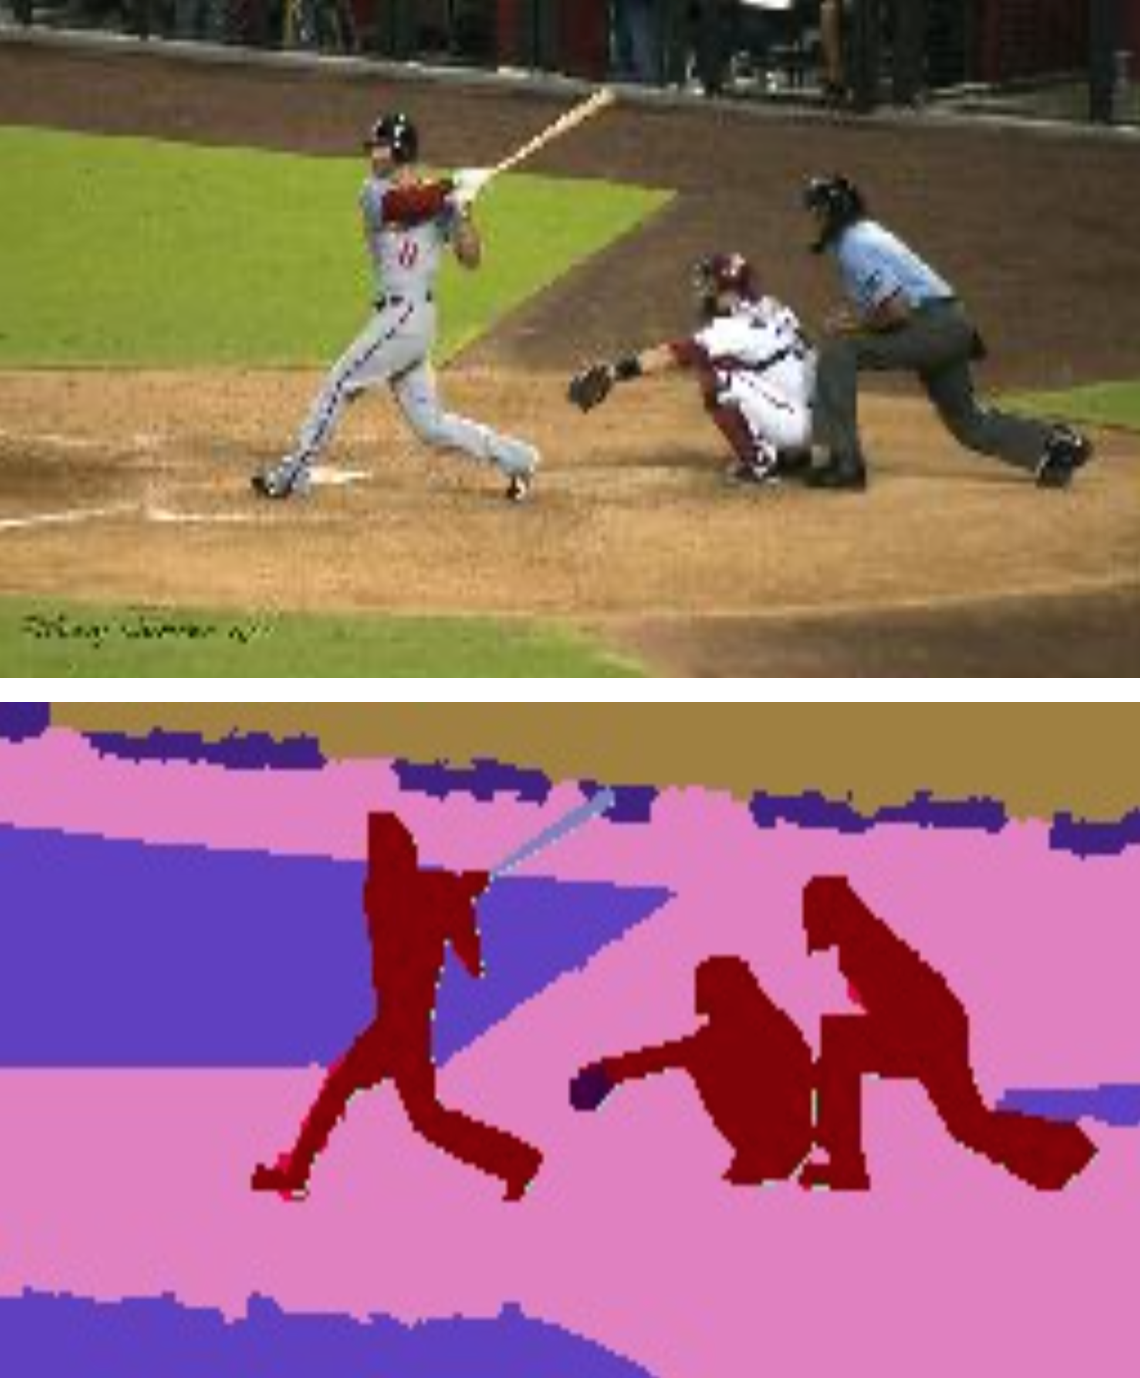
\includegraphics[height=110px]{figures/coco_stuff.png}
            \caption{COCO-Stuff}
        \end{minipage}
        \hspace{0.5cm}
        \begin{minipage}[b]{0.25\linewidth}
            \centering
            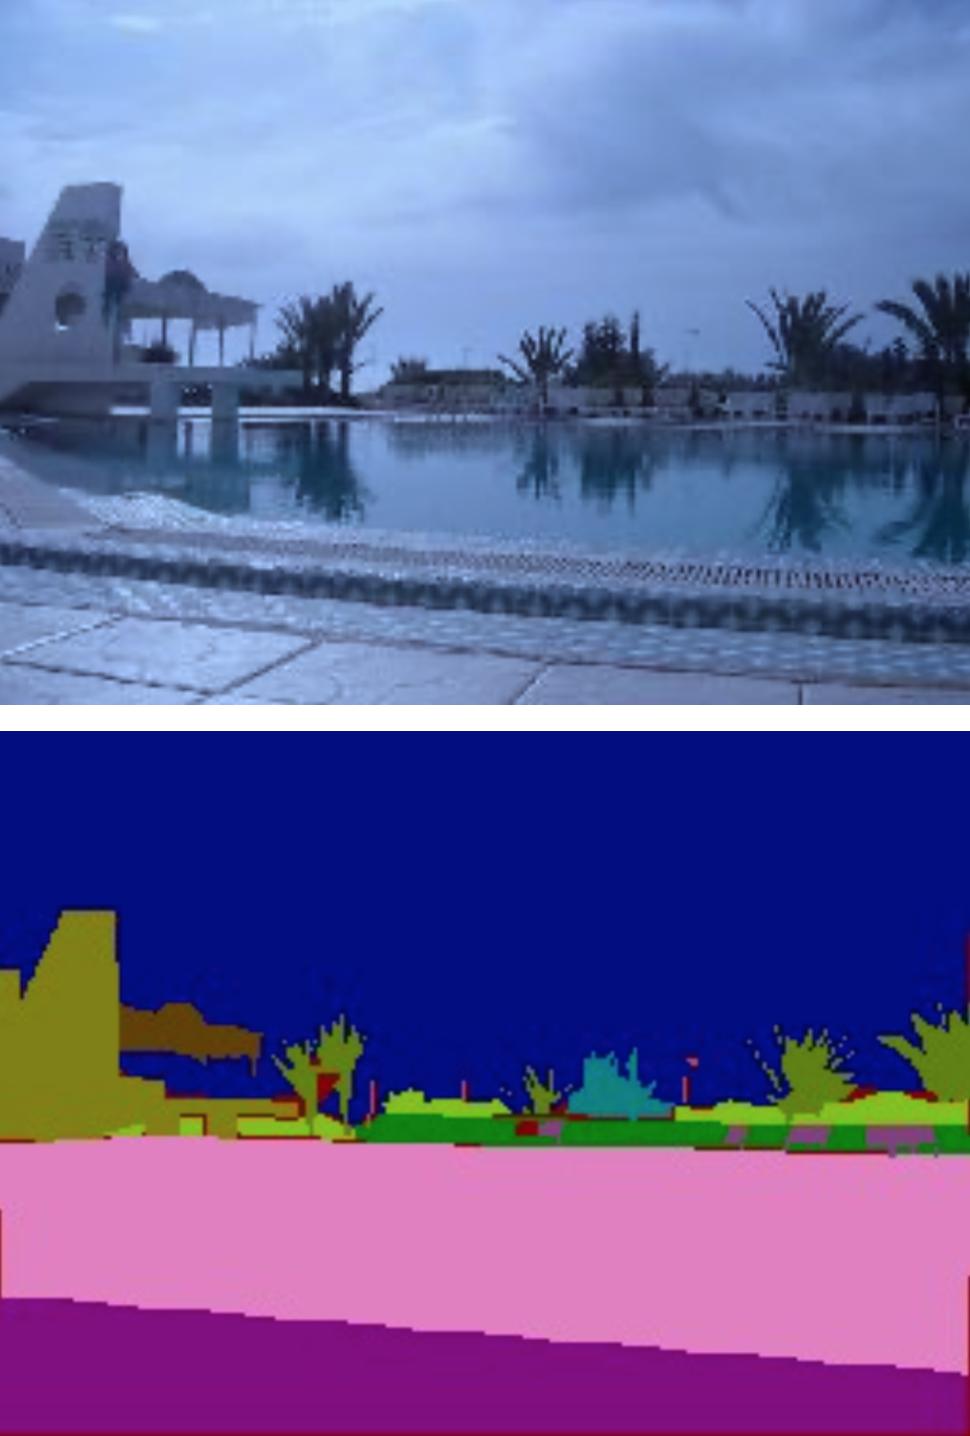
\includegraphics[height=110px]{figures/ade-20k.png}
            \caption{ADE20K}
        \end{minipage}
        \hspace{0.25cm}
        \begin{minipage}[b]{0.33\linewidth}
            \centering
            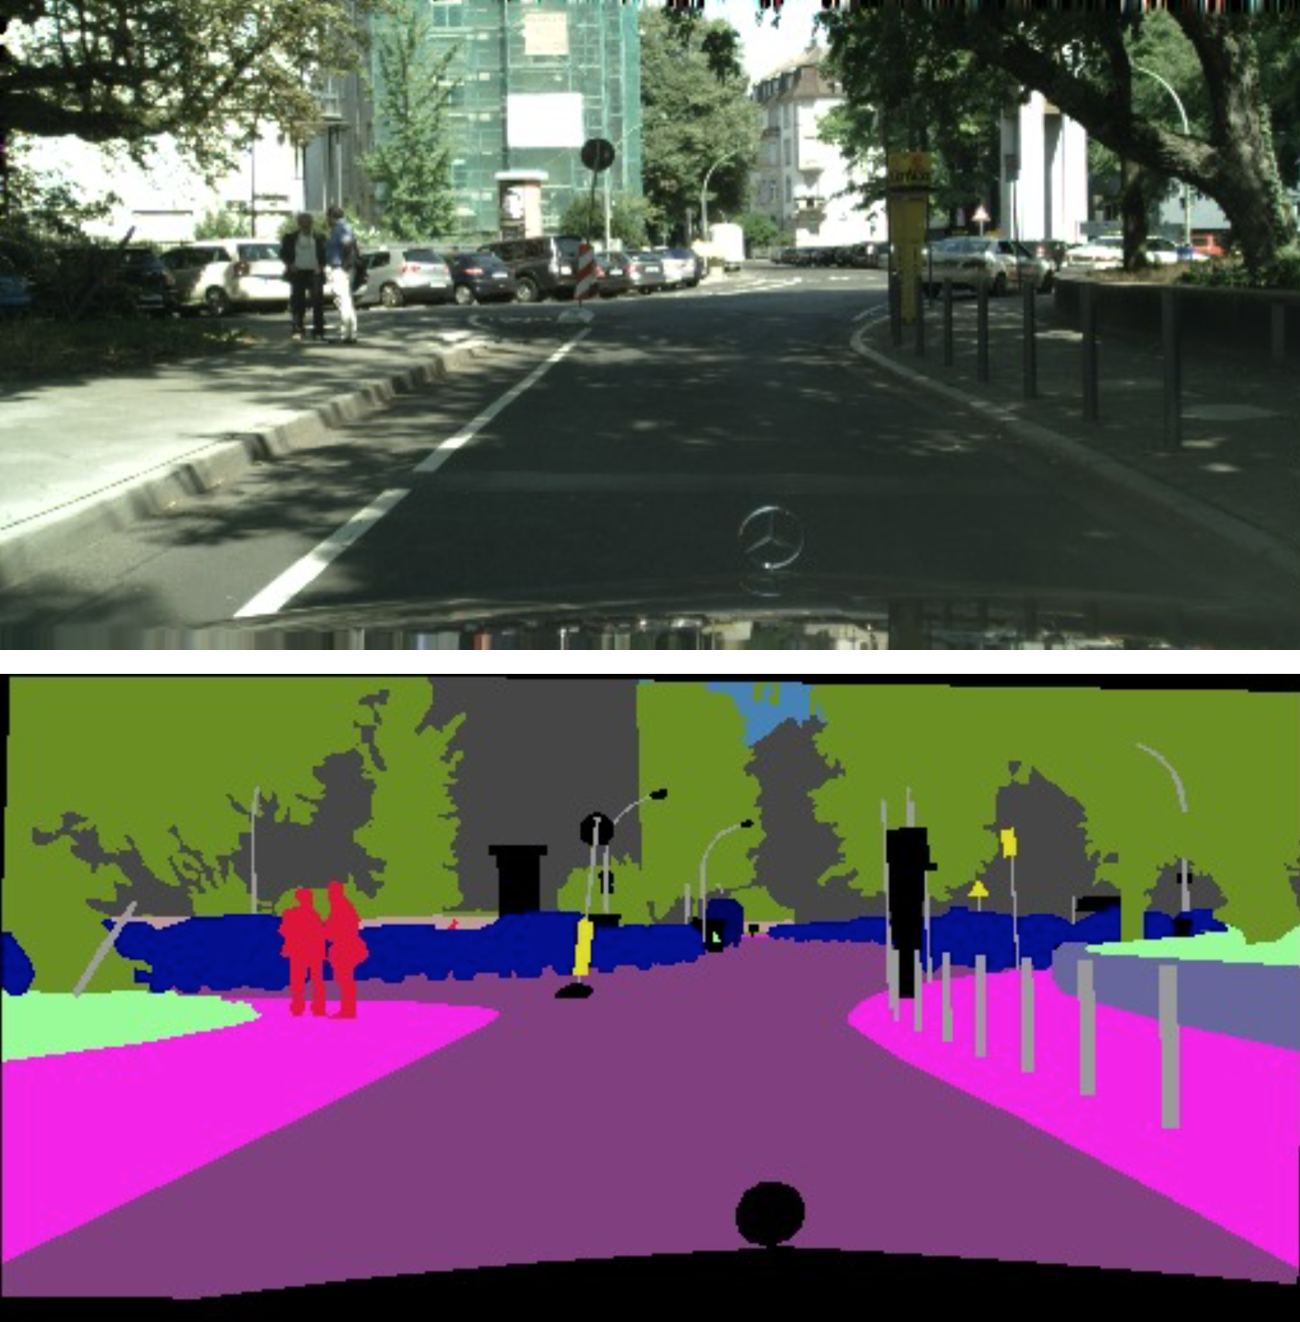
\includegraphics[height=110px]{figures/cityscapes.png}
            \caption{Cityscapes}
        \end{minipage}
    \end{figure}
    
    \begin{table}[]
    \begin{tabular}{|l|l|l|l|l|}
    \hline
    \textbf{Name} & \textbf{Train} & \textbf{Val} & \textbf{Classes} & \textbf{Description}             \\ \hline
    COCO-Stuff    & 118k           & 5k           & 182              & Challenging due to diversity \\ \hline
    ADE20K        & $\approx$20k          & 2k           & 150              & Similar to COCO, very diverse    \\ \hline
    Cityscapes    & 3k             & 0.5k          & 30               & Street scene images              \\ \hline
    \end{tabular}
    \end{table}
\end{frame}

\begin{frame}{Comparison of Qualitative Results}
    \begin{figure}
        \centering
        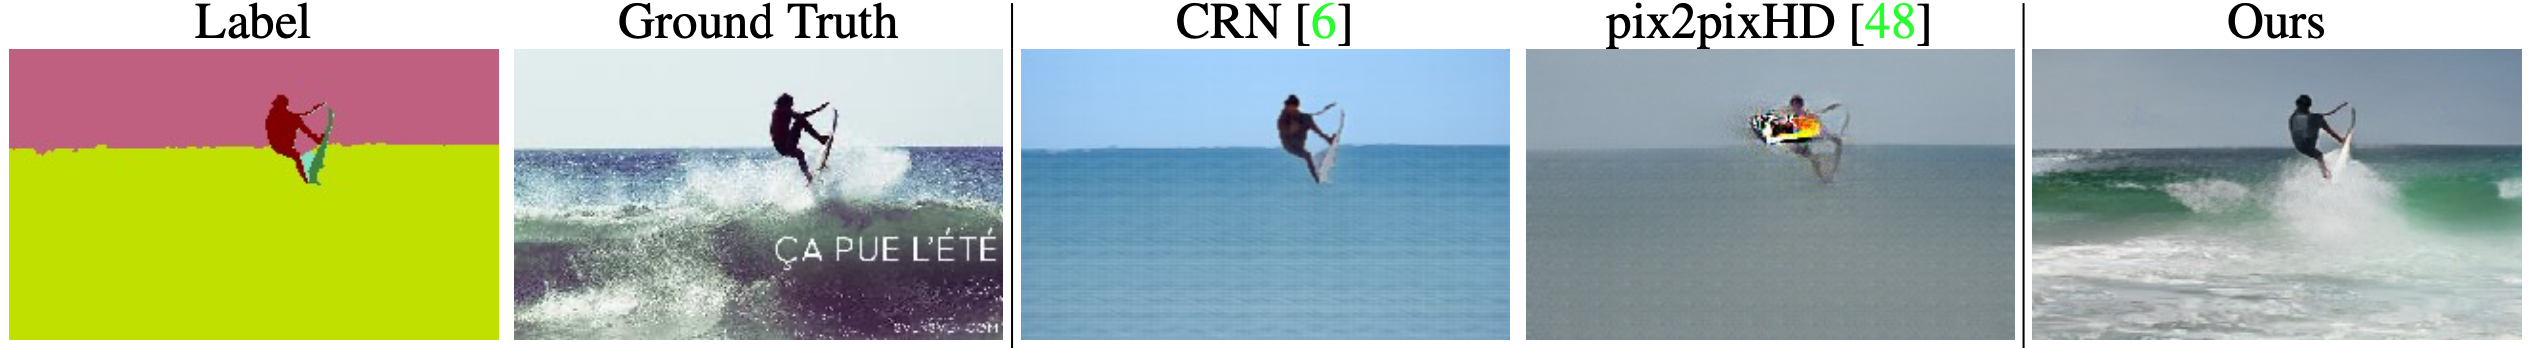
\includegraphics[width=0.93\linewidth]{figures/results_coco.png}
        \vspace{0.3cm}
        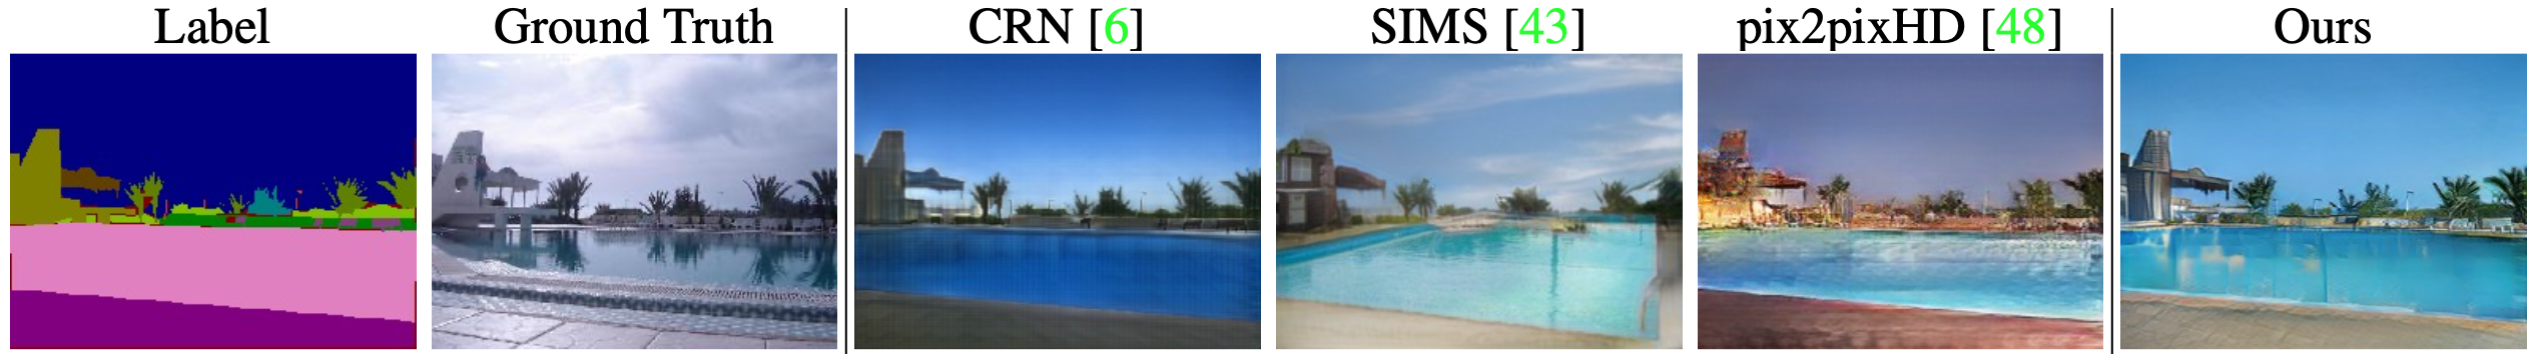
\includegraphics[width=0.93\linewidth]{figures/results_ade-20k.png}
        \vspace{0.3cm}
        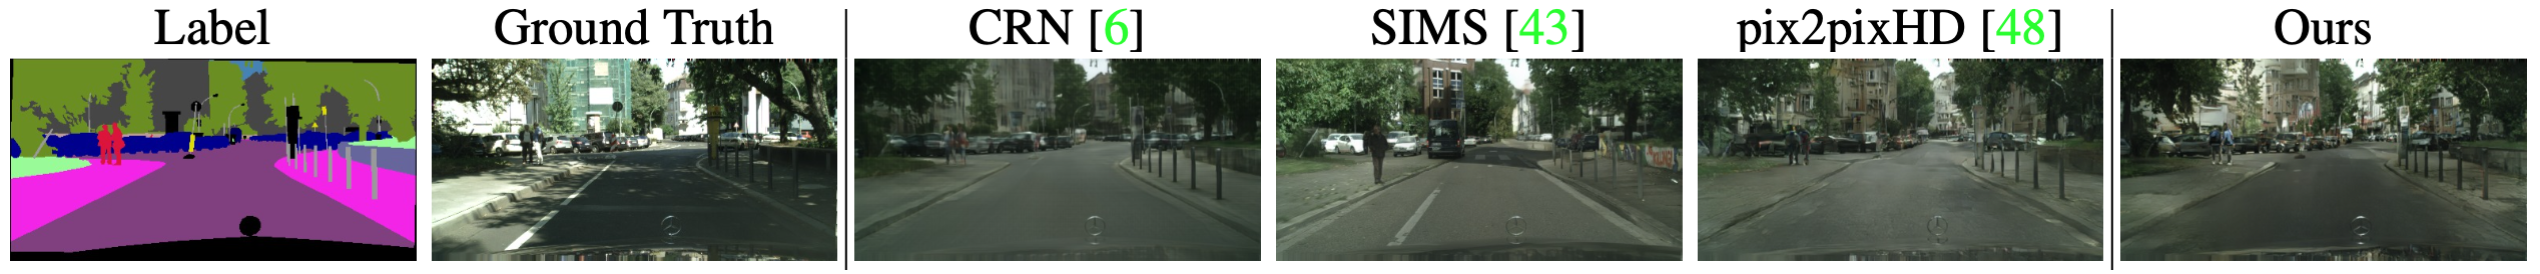
\includegraphics[width=0.93\linewidth]{figures/results_cityscapes.png} 
        \caption{Top: COCO-Stuff, Middle: ADE20K, Bottom: Cityscapes}
    \end{figure}
\end{frame}
% NOTE: no SIMS for COCO-Stuff as it would have been to computationally intensive! 
% NOTE: better visual quality and fewer visible artifacts
% NOTE: SIMS model also renders images with good visual quality. However, the depicted content often deviates from the input segmentation mask (e.g., the shape of the swimming pool)

\begin{frame}{Comparison of Quantitative Results}
    \begin{figure}
        \centering
        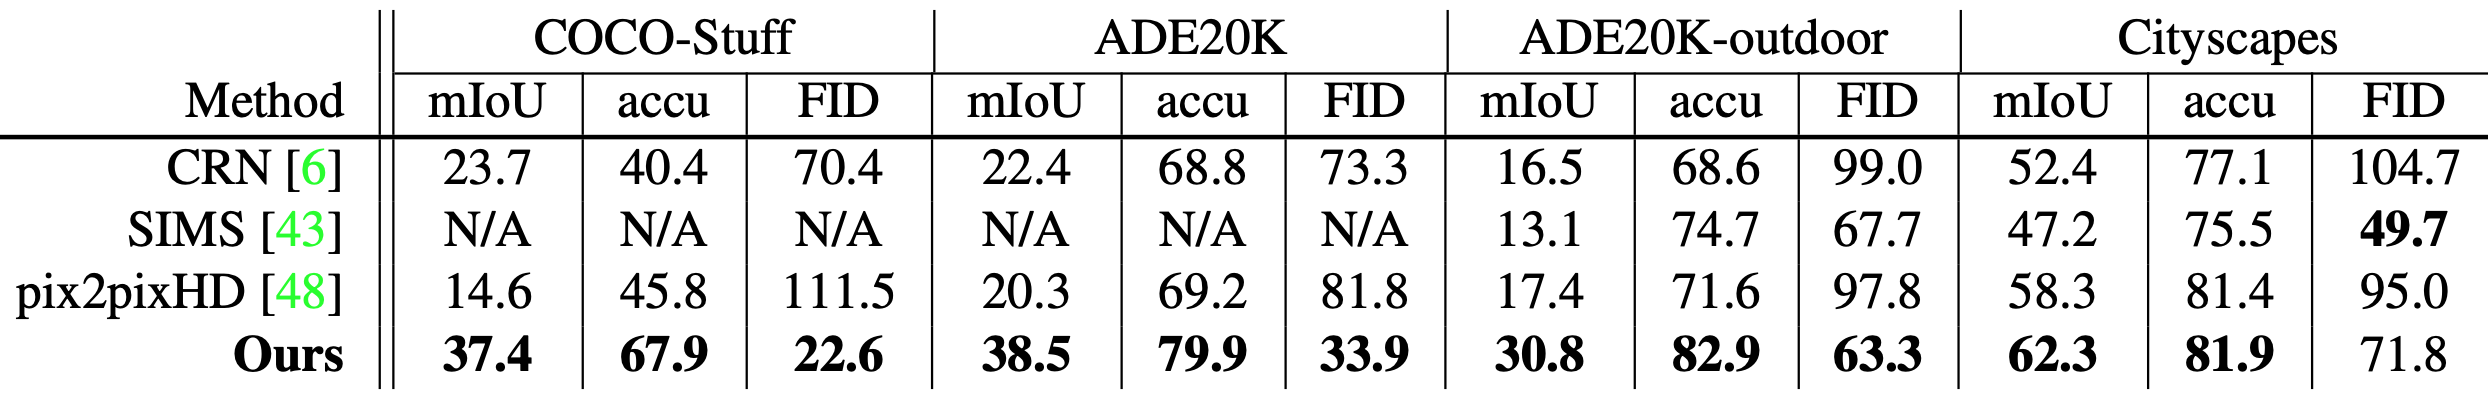
\includegraphics[width=0.93\linewidth]{figures/quant_results.png}
    \end{figure}
    
    \begin{itemize}
        \item Synthesized images are segmented with well-trained models and evaluated with performance metrics
    \end{itemize}
    \begin{enumerate}
        \item \textbf{Mean Intersection over Union}: What is the percentage overlap between predicted and ground truth mask?
        \item \textbf{Pixel accuracy}: What is the percentage of correctly classified pixels?
        \item \textbf{Fr\'{e}chet Inception Distance}: What is the distance between distributions of feature vectors?
    \end{enumerate}
\end{frame}
% NOTE: mIoU: high is good
% NOTE: accu: high is good
% NOTE: FID: low is 
% NOTE: their method outperforms current state-of-the-art methods by a large margin in all the datasets
% NOTE: SIMS --> As using the real image patches, the resulting image distribution can better match the distribution of real images, hence lower FID score but lower mIoU and accu 

\begin{frame}{Why does the SPADE work better?}
\begin{figure}
    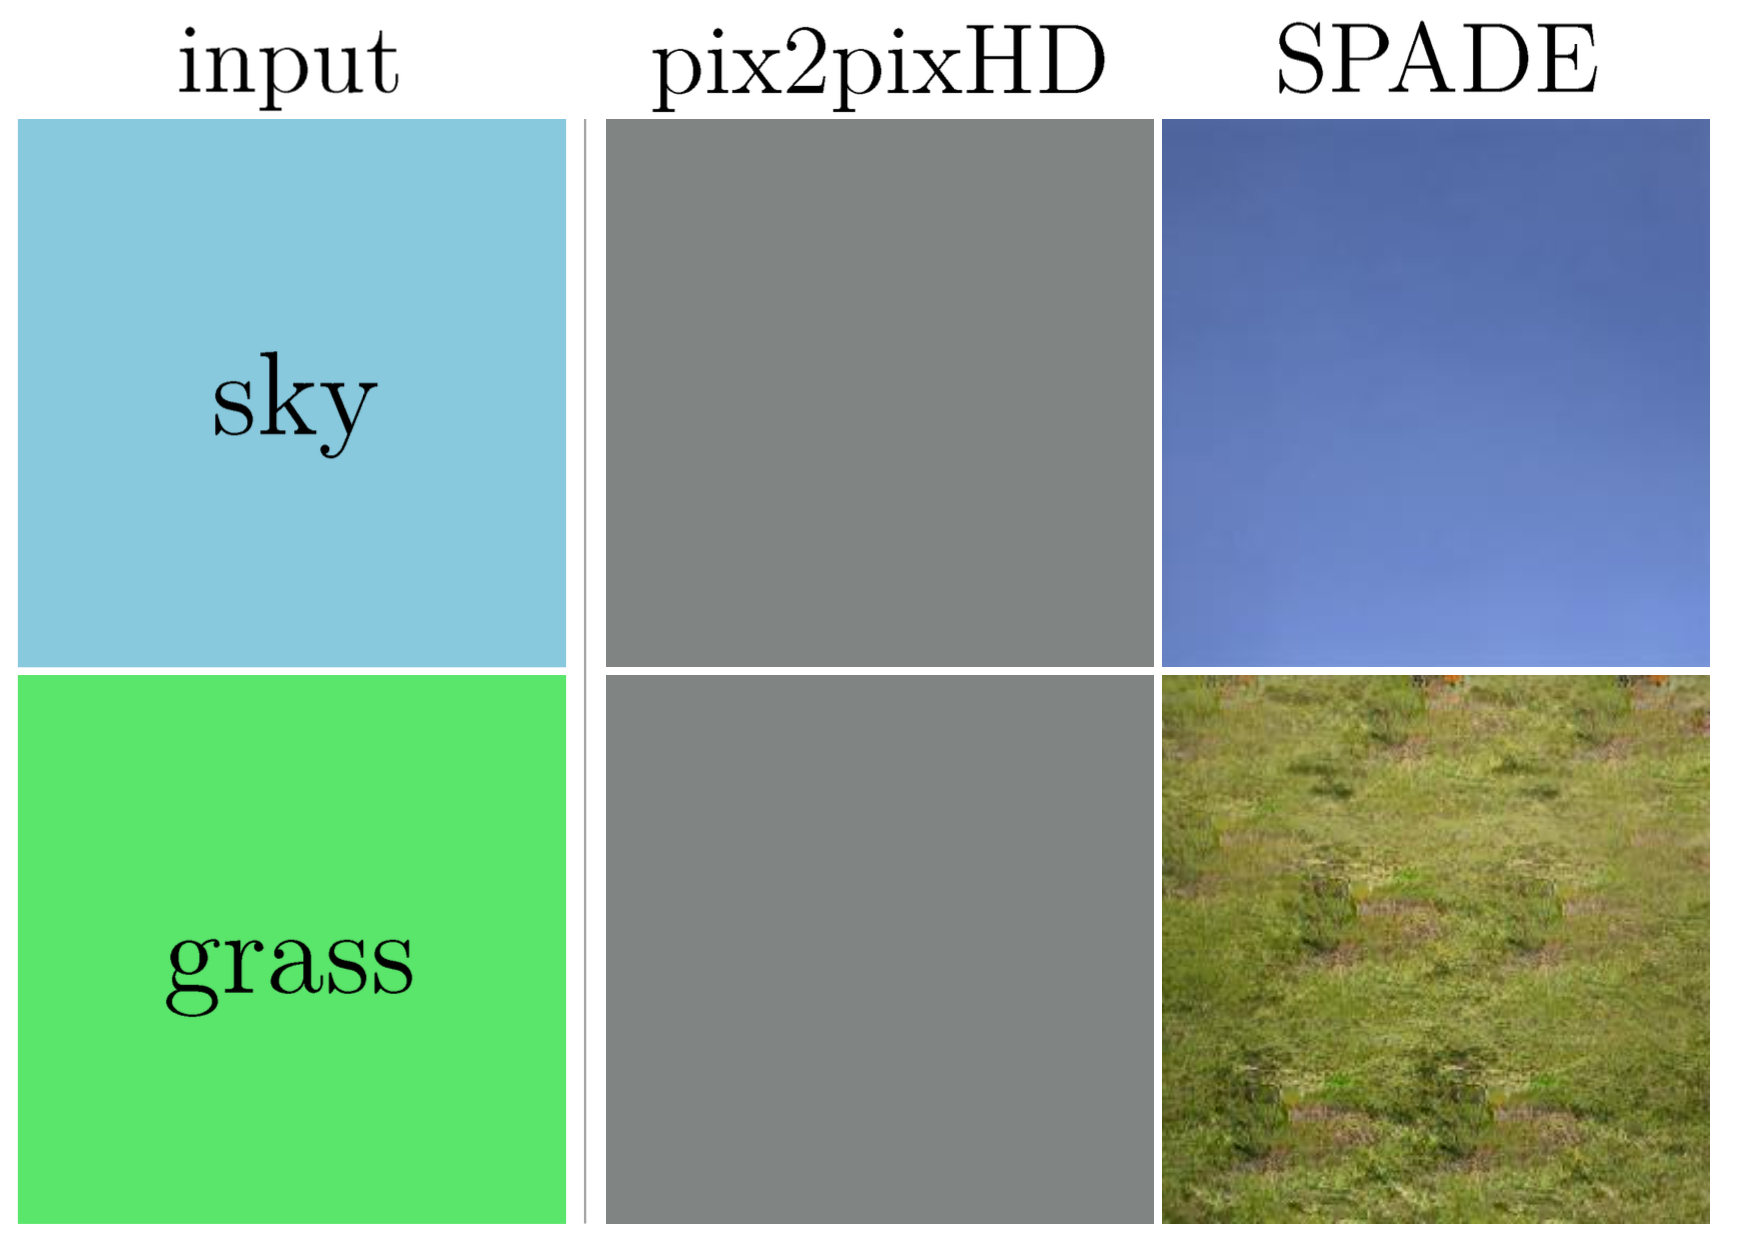
\includegraphics[scale=0.15]{figures/info_loss.png} 
    \caption{Semantic information loss after normalization layer}
\end{figure}
\begin{itemize}[<+->]
    \item Unconditional normalization layers (e.g. InstanceNorm) loose semantic info of uniform masks as \textbf{normalized activations are zero}
    \item SPADE better \textbf{preserves semantic information} because segmentation mask is not normalized but only modulated
    \item SPADE also improves performance of traditional architectures!
\end{itemize}
\end{frame}
% NOTE: "Because a segmentation mask consists of a few uniform regions in general, the issue of information loss emerges when applying normalization"

% CONCLUSION
\section{Conclusion}
\frame{\frametitle{Outline}\tableofcontents[currentsection]}
\begin{frame}{Conclusion}
    \begin{figure}
        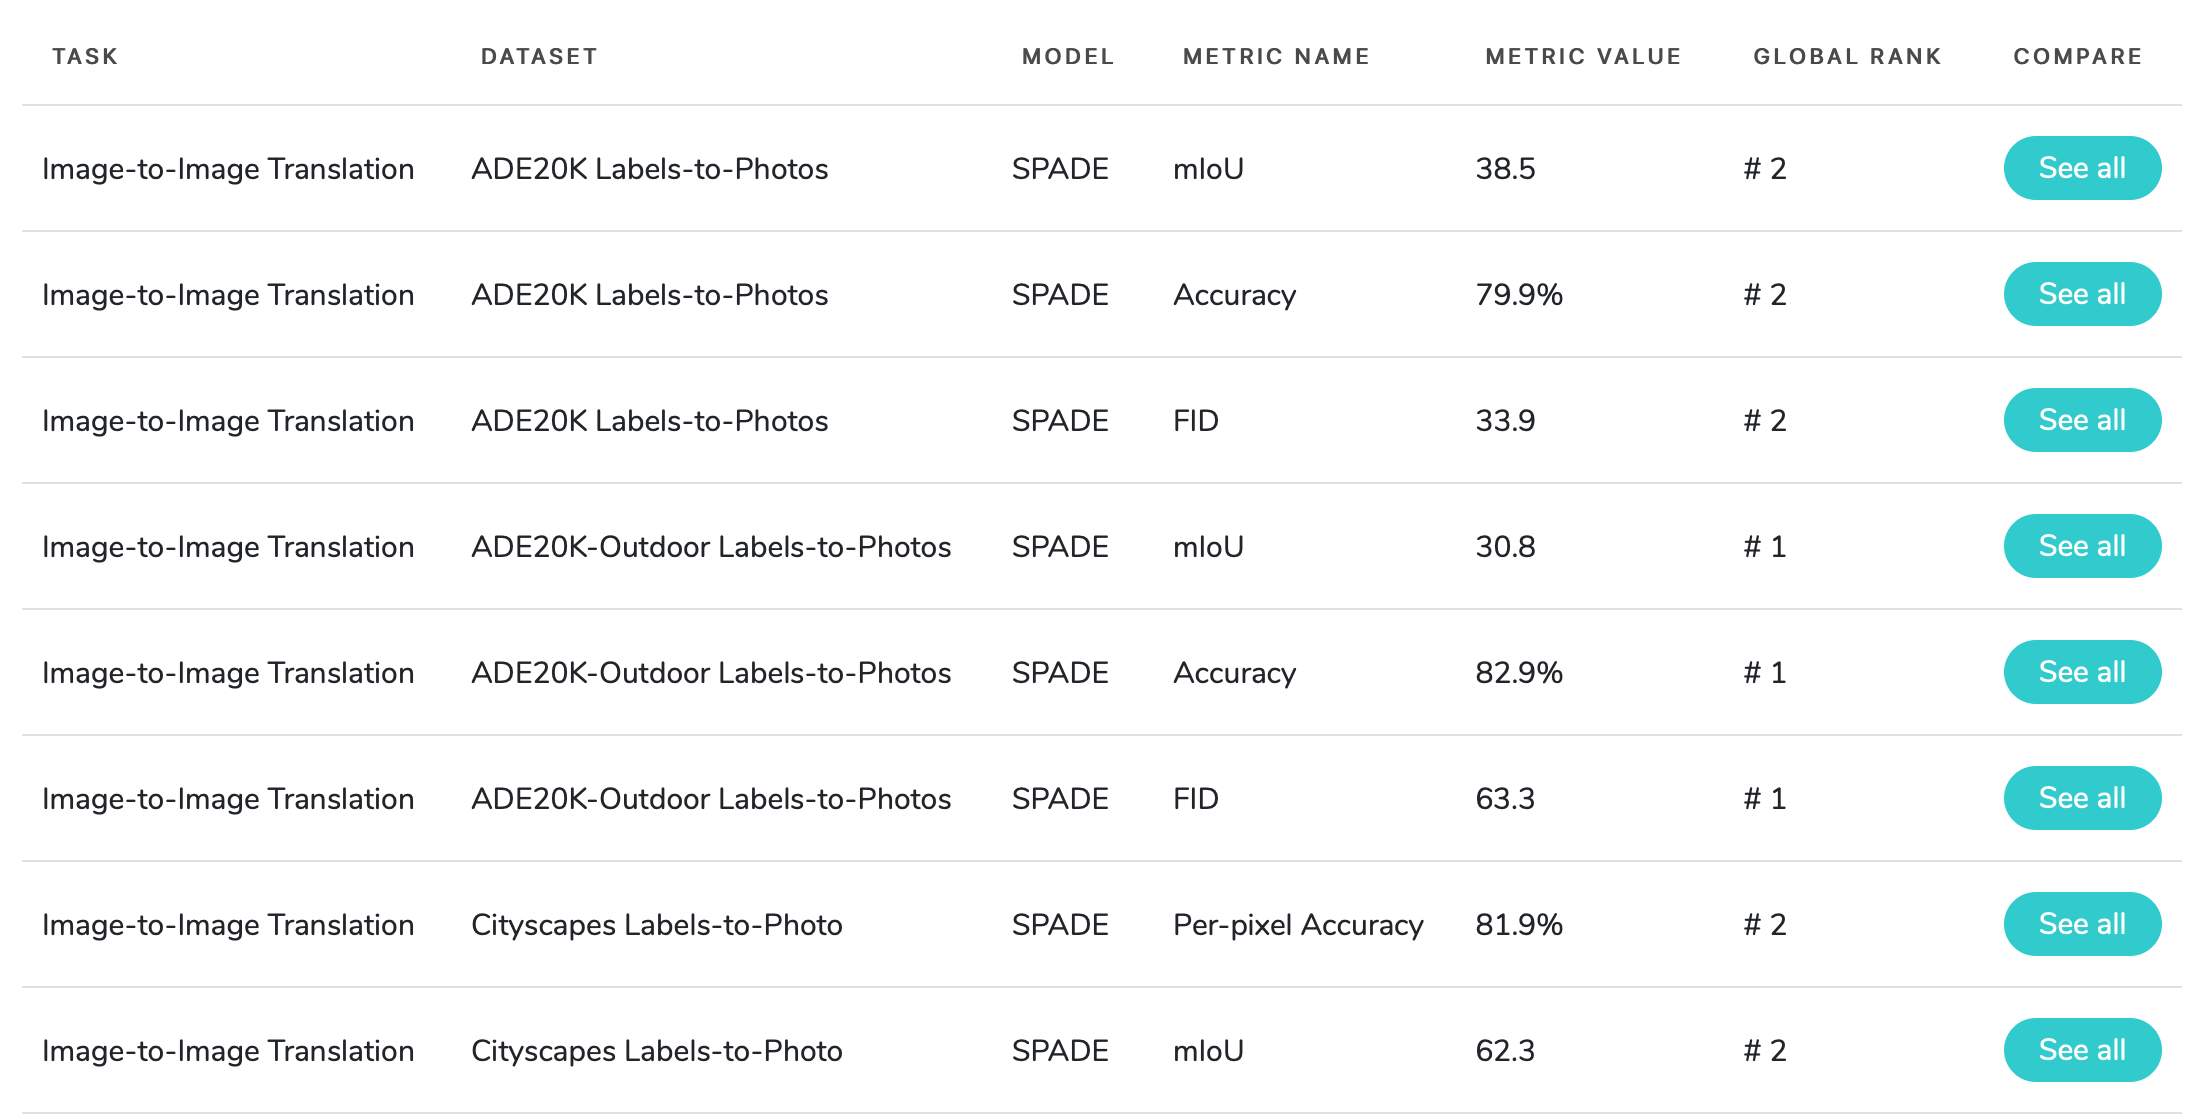
\includegraphics[scale=0.2]{figures/performance.png} 
        \caption{SPADE ranking as of March 2020 \cite{papersWithCode}}
    \end{figure}
    \begin{itemize}
        \item Introduced spatially-adaptive normalization (SPADE) layer
        \item SPADE network outperforms the 2019 state-of-the-art methods by a large margin and is still top-performing (\#1 is \cite{liu2019learning})
    \end{itemize}
\end{frame}

% REFERENCES
\section{References}
\frame{\frametitle{Outline}\tableofcontents[currentsection]}

\begin{frame}[allowframebreaks]
        \frametitle{References}
        \setbeamertemplate{bibliography item}[text]
        \bibliographystyle{abbrv}
        \bibliography{bibliography.bib}
\end{frame}

\end{document}